\documentclass[conference]{IEEEtran}
\IEEEoverridecommandlockouts
\usepackage{cite}
\usepackage{amsmath,amssymb,amsfonts}
\usepackage{algorithmic}
\usepackage{graphicx}
\usepackage{textcomp}
\usepackage{xcolor}
\usepackage{booktabs}
\usepackage{longtable}



\usepackage{url} 
\usepackage{cite}
\usepackage{amsmath,amssymb,amsfonts}
\usepackage{algorithmic}
\usepackage{graphicx}
\usepackage{textcomp}
\usepackage{xcolor}
\usepackage{tikz}
\usepackage{pgfplots}
\usepackage{tabularx}
\usepackage{array}
\usepackage{subcaption}
\usepackage{wrapfig}






\def\BibTeX{{\rm B\kern-.05em{\sc i\kern-.025em b}\kern-.08em
    T\kern-.1667em\lower.7ex\hbox{E}\kern-.125emX}}
\begin{document}

\title{Urban Noise Classification Using Machine Learning Algorithms}


\author{
\IEEEauthorblockN{Javad Ibrahimli\IEEEauthorrefmark{1}, Sena Keleser\IEEEauthorrefmark{1}}
\IEEEauthorblockA{\IEEEauthorrefmark{1}{Electronics and Communications Engineering}, {Istanbul Technical University}, Istanbul, Turkey}
}



\maketitle

\begin{abstract}
The development of Artificial Intelligence day by day creates a new era in technology. As in many fields, artificial intelligence algorithms are used in signal processing and bring innovations to the field of signal processing. In this study it is aimed to classify the noise in voices through artificial intelligence by using data consisting of environmental sounds.\cite{ali2021voice}\cite{verde2018voice} Additionally, it will be examined what results different artificial intelligence models produce.
\end{abstract}

\begin{IEEEkeywords}
Artificial Intelligence, Classification, Noise Classification, Machine Learning, Deep Learning, Data Augmentation, LIBROSA, CNN, LSTM, DNN.
\end{IEEEkeywords}

\section{Introduction}

Urban noise has grown to be a major problem for both policymakers and city inhabitants as an inevitable outcome of urbanization and industry. Noise pollution, also known as the "unseen pollutant," has an adverse effect on people's well-being, healthy and quality of life. One of the biggest environmental risks to public health, according to the World Health Organization (WHO), is noise pollution.\cite{WHO2018} Extended exposure to elevated urban noise levels can result in a range of detrimental health consequences, such as hearing impairment, heart-related disorders, sleep disruptions, and psychological problems like tension and anxiety. Therefore establishing healthier and more pleasant urban environments depends critically on comprehending and reducing urban noise pollution.

Algorithms for machine learning (ML) have become extremely effective at evaluating and understanding vast amounts of data in a variety of fields including environmental monitoring. By automating the noise detection, classification, and analysis processes, machine learning (ML) algorithms provide a number of advantages over classical methods when it comes to urban noise categorization. These algorithms are capable of handling a wide range of complicated information, picking up knowledge from past data and gradually becoming more efficient.\cite{49article}  It is feasible to create reliable and scalable solutions for real-time urban noise monitoring and classification by utilizing cutting-edge machine learning algorithms.


When classifying urban noise using machine learning techniques, signal processing is essential. To preprocess and convert unprocessed audio signals into useful features that may be applied to classification signal processing techniques are utilized.\cite{7891546} These features frequently consist of the audio signals' time-domain and frequency-domain properties, such as amplitude, power spectral density, and Mel-frequency cepstral coefficients (MFCCs). Wavelet transforms and short-time Fourier transforms are examples of advanced signal processing techniques that can further improve the relevance and quality of the retrieved features, increasing the accuracy of noise classification models. \cite{musicclassificationarticle}

Furthermore, the automation and scalability of ML models enable their widespread deployment throughout vast metropolitan regions with little to no human involvement. Noise monitoring becomes more effective and economical as a result of the decreased dependence on manual data collection and processing. Moreover ML-based noise classification systems can encourage community involvement, and support for noise reduction activities by increasing public awareness of noise pollution and its impacts through the provision of transparent and easily accessible noise data.\cite{vijayakumar2022ecg}


Classifying urban noise using machine learning techniques is still a relatively new topic with a lot of room for development. The accuracy and resilience of noise classification models can be strengthened in the future and ML can be integrated with other technologies like edge computing and the Internet of Things (IoT) and new use cases like noise prediction and simulation can be investigated.\cite{8300941} Furthermore, the efficiency and influence of ML-driven noise control solutions can be increased by interdisciplinary partnerships between computer scientists, urban planners, public health specialists and legislators.


The following sections of this report will take the readers
through an in-depth background and related work and explaining the state of the art; implemented algorithms which will detail the dataset, algorithms, code, system setting, and key performance indicators 
methodologies used; followed by results and discussion on the
challenges we faced during the project’s fruition. Lastly, we
will meet the clarion call of future work, promising to further
grow the field of Urban Noise Classification Process.

\\

\section{Background and Related Work}
Albaji et al.(2023) conducted a study on noise pollution mapping in urban using machine learning algorithms.\cite{albaji2023investigation} They implemented different types of algorithms to map, and classify noises in voices aiming to provide a comprehensive assessment of urban noise pollution.\cite{tandel2020voice} They have implemented machine learning to predict noise pollution patterns to data which is collected by themselves from different urban areas. The study demonstrates the effectiveness of machine learning algorithms in noise classification.

Ali, Rashid, and Hamid (2022) studied machine learning algorithms to classify environmental noise in smart cities.\cite{r1} They implemented a system that collects data, processes it using feature extraction methods and applies different machine learning algorithms to classify different types of urban noise. This paper highlights the possibilities of to managing and mitigating noise pollution in smart cities using machine learning.\cite{boonprong2018classification}

A one research studied by Renaud et al.(2023) explored making long-term predictions of noise levels based on data collected in a English city. They implemented several deep learning models (Transformer,TFT,CNN-LSTM,LSTM), and Gradient Boosting algorithms and obtained long-term and short-term predictions. Also this paper proposes an approach for detecting noise level anomalies based on predictions. \cite{RENAUD2023119568}

The UrbanSound8K dataset which is also included in this paper, was utilized by Bubashait and Hewahi (2021) to compare the performance of Deep Neural Networks (DNNs), Convolutional Neural Networks (CNNs), and Long Short-Term Memory (LSTM) networks. This collection of recordings of urban sounds provides a standard against which to compare different machine learning models.\cite{gupta2019dealing} They found that while DNNs are very good at handling structured data, they have trouble with temporal dependencies; CNNs are very good at extracting spatial features from audio spectrograms; and LSTMs are very good at capturing the temporal patterns within sequential data. The thorough comparison revealed that although CNNs were generally better at learning hierarchical features, LSTMs were also able to achieve competitive results by using their ability to represent long-term dependencies in audio signals. The significance of choosing suitable neural network designs depending on the particulars of the dataset and the type of classification task is highlighted by this comparative analysis.\cite{bubashait2021urban}



Zambon et al. (2018) explored methods for monitoring and predicting traffic noise in large urban areas.\cite{app8020251} They developed models to analyze noise data, providing insights into current noise levels and predicting future trends. This research supports urban noise management by enabling more informed decision-making and effective mitigation strategies. The study demonstrates the importance of integrating monitoring systems with predictive analytics for improved urban noise control. \cite{50article}



\section{Implemented Algorithms}
\subsection{Deep Neural Networks}
One of the most fascinating innovations in artificial intelligence is the neural network which draws inspiration from the human brain. \cite{128859190} Deep neural networks (DNNs) have shown amazing performance in a range of complex tasks which has transformed numerous fields, including natural language processing, speech recognition and computer vision. Through numerous layers of nonlinear transformations, DNNs can automatically learn hierarchical representations of data, which is what gives them their power. This feature makes it possible for DNNs to effectively describe complex patterns and dependencies in data that are difficult for traditional machine learning algorithms to capture.\cite{samek2021explaining}

As seen in Fig \ref{fig:dnnstructure}. three layers make up a standard DNN: an input layer, several hidden layers, and an output layer.\cite{cichy2019deep} Neurons which make up each layer are linked to neurons in layers above and below. Weights are connected with the connections between neurons and are acquired during training. In order to reduce the error between the goal values and the predictions made by the network, these weights must be adjusted during the learning process. The backpropagation algorithm is usually used for this, computing the gradient of the loss function with respect to each weight and updating the weights based on the result.

\begin{figure}[htbp]
\centerline{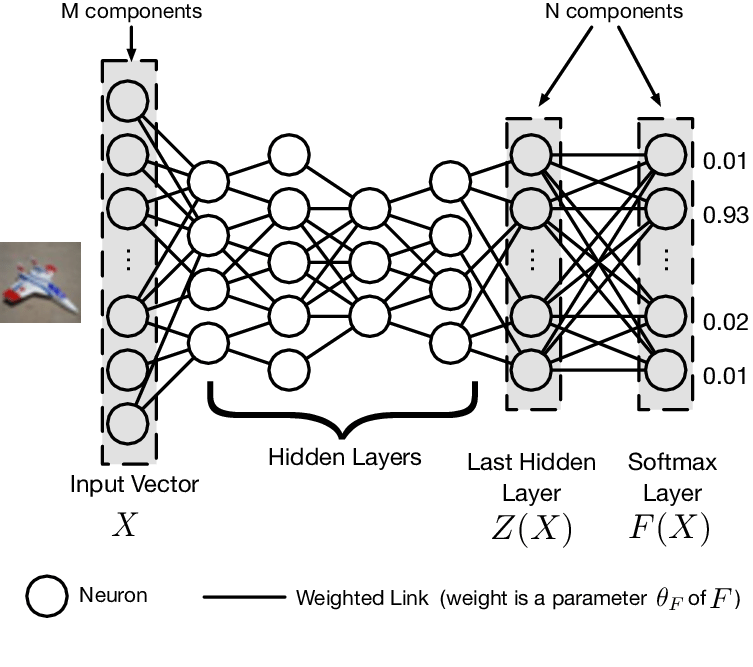
\includegraphics[width=0.5\textwidth]{Images/dnnstructure.png}}
\caption{Overview of a DNN architecture: This architecture, suitable for classification tasks thanks to its softmax output layer, is used throughout the paper along with its notations. \cite{article}}
\label{fig:dnnstructure}
\end{figure}

The capacity of DNNs to learn hierarchical representations is one of their main advantages.\cite{samek2021explaining} Generally, a DNN's upper layers catch more abstract properties like objects or shapes, while its bottom layers record low-level features like edges in an image. DNNs may construct complex features from smaller ones through this hierarchical learning process, which is essential for jobs requiring high-dimensional data interpretation. \cite{highperformanceinproceedings}

Practical applications of DNNs are significantly impacted by how well they process data. It makes it possible to implement complicated models on devices with limited resources, like edge computing platforms, IoT devices, and smartphones. For real-time applications where latency and power consumption are important considerations, such as autonomous driving, this is vital.\cite{sze2017efficient} Furthermore, by lowering operating costs and energy consumption, effective processing methods enable the use of DNNs in large-scale applications, like cloud-based services and data centers.\cite{BODDAPATI20172048}

\subsection{Random Forest}
Random Forest is a classification approach that creates an ensemble using many univariate classification trees as a complicated composite classifier.\cite{agjee2018impact} The ensemble learning technique known as Random Forest has become very popular because of its precision,dependability and user-friendliness. Leo Breiman first presented it in 2001, and since then, it has grown to be one of the most effective and adaptable machine learning techniques.\cite{rigatti2017random} Decision trees are basic, understandable models that divide the feature space into discrete areas according to the characteristics of the input data. The Random Forest algorithm expands on this idea. Decision trees can be highly variable and prone to overfitting, but Random Forest uses ensemble learning to reduce these problems.

Essentially, a Random Forest is made up of several decision trees that were built using various subsets of the training set as seen in Fig\ref{fig:RF}. In order to guarantee that every tree is trained on a distinct set of observations, this procedure, referred to as bootstrapping, entails sampling the data with replacement. Additionally, only a random subset of features is taken into account when splitting nodes during the building of each tree. By adding another layer of randomness, this improves the model's resilience and capacity for generalization by decorrelationing the trees. \cite{phdthesis1}
\begin{figure}[htbp]
\centerline{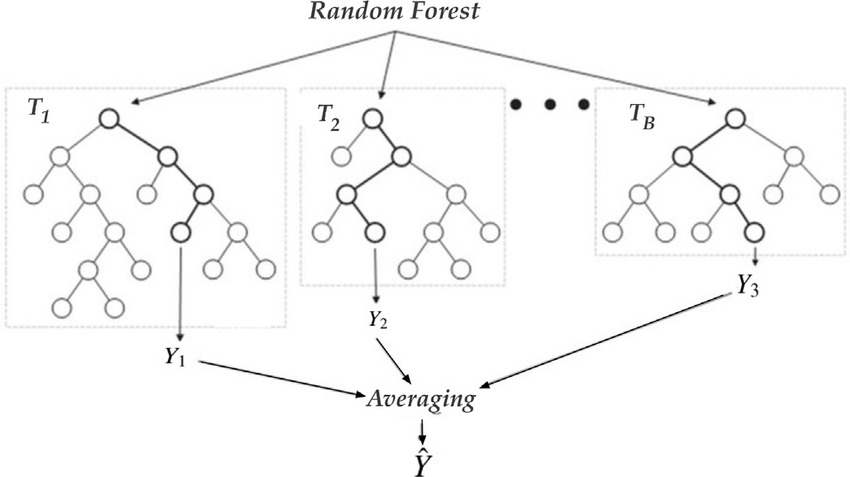
\includegraphics[width=0.5\textwidth]{Images/RFstructure.jpg}}
\caption{Random Forest structure \cite{agjee2018impact}}
\label{fig:RF}
\end{figure}

Random Forests are popular because of a number of appealing characteristics. They can handle both numerical and categorical data without requiring a lot of preprocessing, and they can handle huge datasets with high-dimensional features.\cite{biau2016random} Additionally, the technique withstands data noise and outliers rather well. Random Forests can also be used to evaluate each feature's significance for the prediction process. A metric of feature relevance can be obtained by examining the decrease in impurity (such as entropy or Gini impurity) that each feature across all trees contributes. This is very helpful for performing feature selection and comprehending the underlying data structure.



\subsection{Long Short Term Memory(LSTM)}

A kind of recurrent neural network (RNN), Long Short-Term Memory (LSTM) networks have emerged as a keystone of deep learning, especially for tasks involving sequential input. In order to overcome the drawbacks of conventional RNNs, particularly the vanishing gradient issue, Hochreiter and Schmidhuber invented LSTMs in 1997. \cite{dipietro2020deep} RNNs have difficulty learning long-term dependencies because of this issue, which arises when gradients employed in training drop exponentially as they propagate back over time.

Fig\ref{fig:LSTM} depicts the general architecture, and the setup specifics of the LSTM hyperparameters are presented below.Effective maintenance and updating of long-term dependencies is made possible by the distinct cell structure incorporated into LSTM networks. Input, forget, and output gates are the three main gates found in each LSTM cell.\cite{kawakami2008supervised} By regulating the information flow into, through, and out of the cell, these gates help the network to hold onto useful data for longer periods of time while removing unnecessary data.

\begin{figure}[htbp]
\centerline{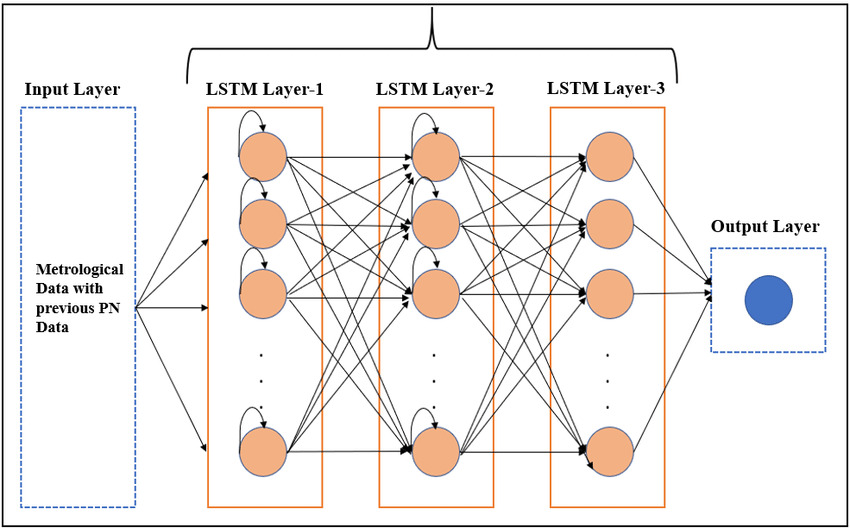
\includegraphics[width=0.5\textwidth]{Images/LSTM.jpg}}
\caption{Sequential Long Short-Term Memory (LSTM) architecture. \cite{LSTM}}
\label{fig:LSTM}
\end{figure}

Capturing long-term dependencies is a vital capability of LSTM networks and is one of its key advantages for many sequential data applications. For example, long short-term memory (LSTM) is utilized in natural language processing (NLP) for tasks like language modeling, machine translation, and text production, where semantic sequence maintenance and context awareness are very important.\cite{dipietro2020deep} Likewise, long short-term memory banks (LSTMs) have considerable utility in the financial, meteorology, and medical fields because they can forecast future values in time series analysis by using existing data. \cite{lstmarticle}

LSTMs have demonstrated great potential in the urban sound classification setting because of their capacity to gradually learn and identify patterns in audio data.\cite{lezhenin2019urban} Urban sound classification is a difficult problem because it requires separating out and classifying a wide range of sound events from complex and chaotic acoustic settings, such as human activities, road noise, and construction sounds. The temporal dependencies included in audio data, which are crucial for differentiating between different kinds of sounds, are frequently difficult for traditional sound classification techniques to capture.

\subsection{Convolutional Neural Networks (CNN)}
Deep learning has been transformed by Convolutional Neural Networks(CNN), especially in the area of classification tasks. They are highly useful for usage in a wide range of applications due to their ability to automatically and adaptively learn spatial hierarchies of features from input data.\cite{lu2021review} CNNs play a key role in accurately classifying traffic patterns and detecting anomalies in the field of traffic anomaly detection in Internet of Things networks.

According to Kang et al., CNNs perform well while managing missing data, which is a typical problem in a lot of real-world Internet of Things applications. They suggest a deep similarity metric approach that makes use of CNNs to extract pertinent characteristics from traffic data, improving anomaly detection. It has been observed that CNNs' convolutional layers have the ability to identify local dependencies in the data, which is very helpful in deciphering intricate traffic patterns.\cite{CNN}


\begin{figure}[htbp]
\centering
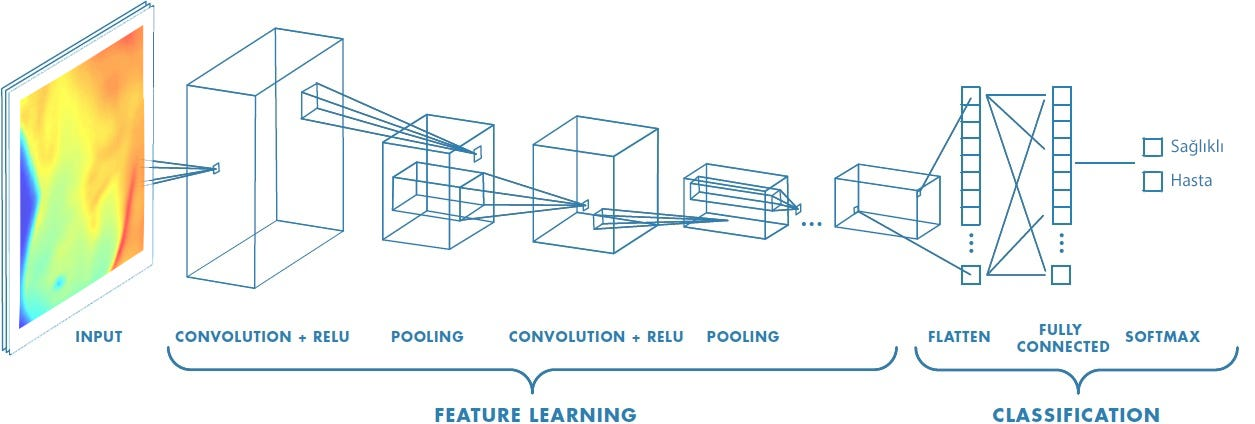
\includegraphics[width=0.5\textwidth]{Images/cnn.jpg}
\caption{Architecture of a Convolutional Neural Network (CNN). The traditional CNN structure is mainly composed of convolution layers, pooling layers, fully connected layers, and some activation functions. Each convolution kernel is connected to the part of feature maps. The input is connected to all of the output elements in the fully connected layer. \cite{CNN}}
\label{fig:CNN}
\end{figure}

A standard architecture  for a CNN is given \ref{fig:CNN}includes a number of layers: convolutional layers, pooling layers, and fully connected layers. Convolutional layers apply filters to the input data to produce feature maps, highlighting important patterns \cite{CNN}. Pooling layers proceed to decrease the dimensionality of these feature maps, retaining the most important information while reducing the computational load. Fully connected layers amalgamate the features extracted for either prediction or classification purposes, thereby completing the classification process.

Convolutional Neural Networks have demonstrated exceptional performance in the noise classification domain, particularly in the task of identifying sounds in cities.\cite{bubashait2021urban}\cite{song2021machine} One may argue that CNNs are capable of automatically extracting and learning hierarchical characteristics from unprocessed audio data, which are essential for differentiating between various urban noise classes. According to Bubashait and Hewahi's study, CNNs are particularly good at handling the spectrum representation of audio inputs. CNNs can identify and categorize sound patterns with high accuracy by using their spatial hierarchies to convert unprocessed audio data into spectrograms. By combining the best features of image recognition with audio classification, this transformation enables CNNs to bridge the gap between visual and aural data processing methods.


\section{Methodology}

The 8,732 tagged sound snippets from 10 different classifications (air conditioner, vehicle horn, children playing, dog barking, drilling, engine idling, gunshot, jackhammer, siren, and street music) that are 4 seconds or less in length make up the UrbanSound8K dataset. Using a variety of machine learning models, including Random Forest, Deep Neural Networks, Convolutional Neural Networks, and Long Short-Term Memory Networks, the objective is to categorize these sounds according to their properties. The current methodology outlines the general procedures required to pre-process the data, extract significant features, choose and use suitable algorithms, and assess their effectiveness.

The process begins with the loading of data. The UrbanSound8K dataset's audio files and metadata are all imported. Data cleaning is carried out in order to handle any missing or corrupted audio files and make sure that all audio files have the same sampling rate and are in the same format (e.g.,.wav files). Techniques for reducing noise are used to improve the quality of the audio signals; they may include leveling audio levels or filtering out background noise. To ensure a thorough review, it is then separated into training, validation, and test sets, usually at a ratio of 70\% for training, 15\% for validation, and 15\% for testing.

Converting audio data into a format that machine learning algorithms can understand requires a step called audio feature extraction. Mel-frequency Cepstral Coefficients, which describe the audio signal in a compact form and capture the sound's power spectrum, are among the often retrieved features. \cite{spectogramissuesarticle} It is possible to identify musical elements in the audio by using chromagram characteristics, which stand for 12 distinct pitch classes. The timbre texture of a sound is captured by spectral contrast, which quantifies the amplitude difference between peaks and troughs in the spectrum. When differentiating between tonal and noisy signals, the Zero-Crossing Rate is used to evaluate how quickly a signal changes sign. Aside from that, Root Mean Square is used to assess the audio signal's energy, which gives information about its volume.

Next, decide which machine learning algorithms are best for classifying the audio data. Given that the characteristics have been acquired, the DNN, CNN, Random Forest, and LSTM algorithms are suitable for this task due to their efficaciousness in handling audio data. 


\begin{figure*}[htbp]
\centerline{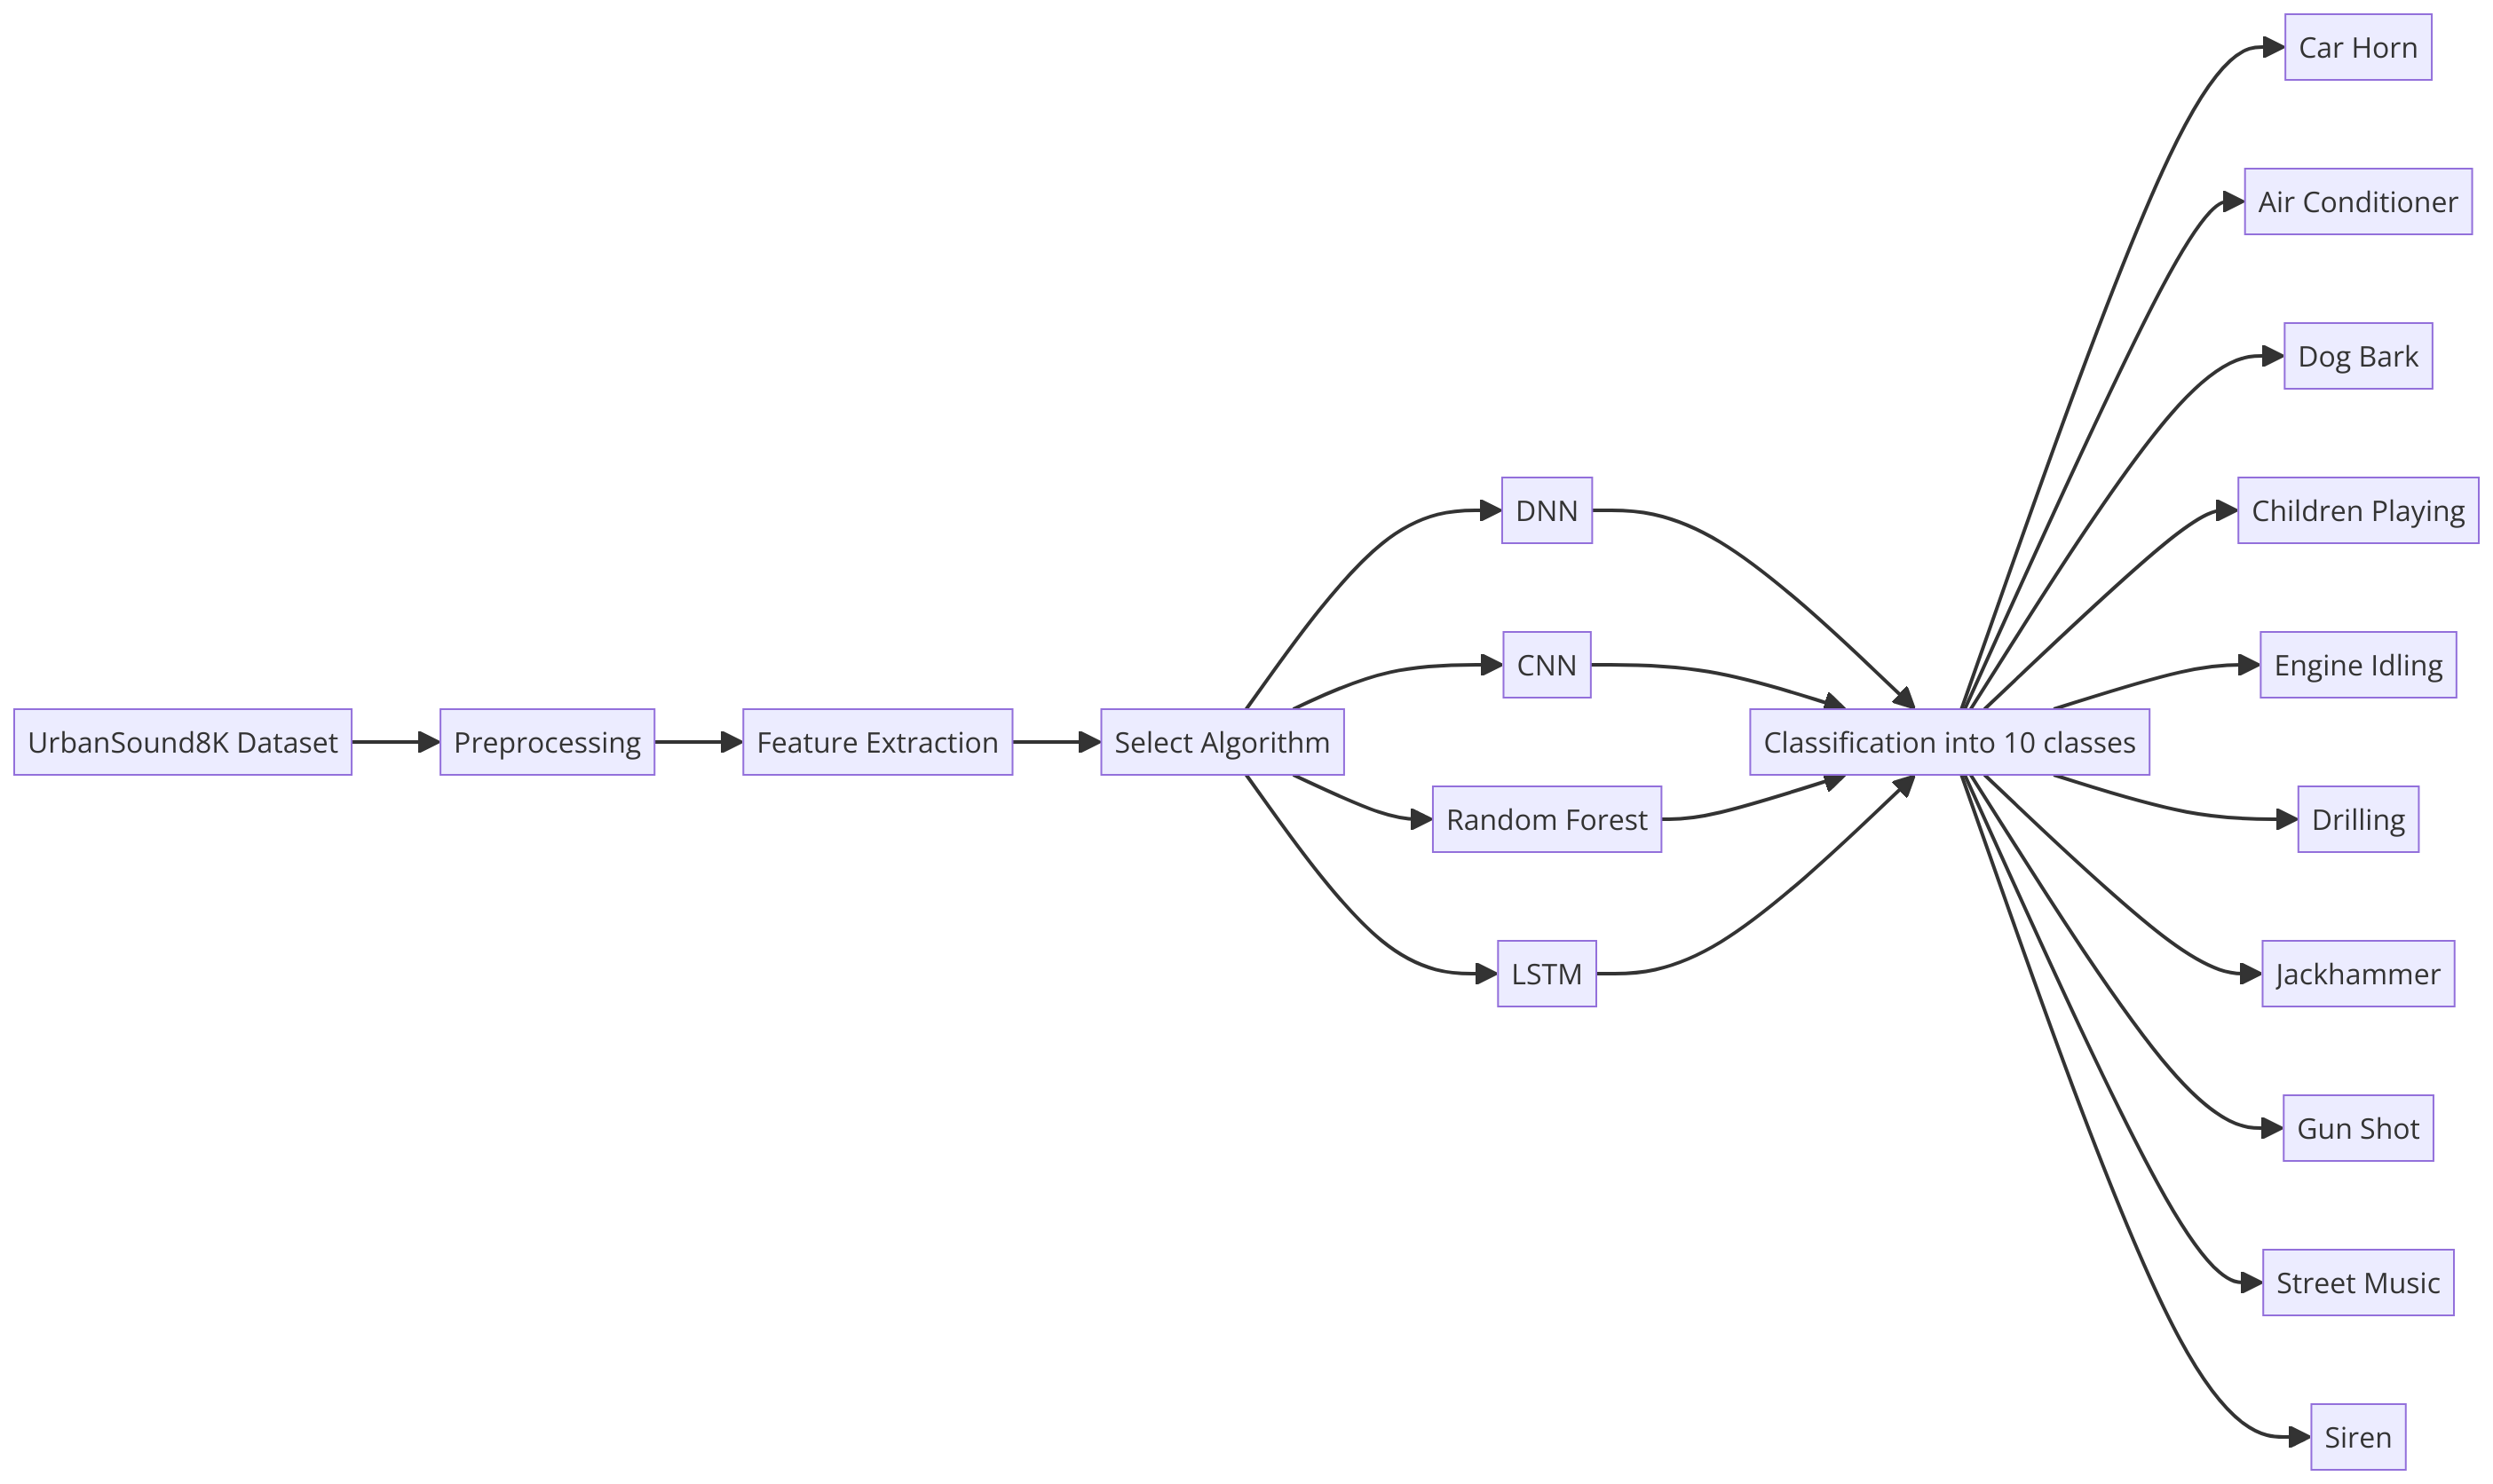
\includegraphics[width=0.8\textwidth]{Images/diagram.png}}
\caption{Process Flowchart}
\label{fig:farmer}
\end{figure*}

Fully connected neural networks, or DNNs, may be a suitable choice for extracting high-level abstractions from the information. CNNs can be used to create spectrograms or other image-like feature representations because they are good at capturing spatial hierarchies in the data.\cite{algan2021image} A type of ensemble learning called Random Forest is resistant to overfitting and operates by building several decision trees. Recurrent neural networks, such as long short-term memory (LSTMs), are useful for modeling time-series audio properties because they can extract temporal dependencies from sequential data. \cite{rawarticle}

The input features of CNN and DNN models are normalized, and the number of layers and neurons in each layer of the network architecture is set initially. The models are then optimized for hyperparameters based on the validation set performance, and trained using the Adam optimizer and categorical cross-entropy loss function. Using bootstrapped samples of the training data, numerous decision trees are trained for the Random Forest, and a majority voting method is used to combine the predictions from the many trees into a single forecast. To use LSTM, input features must be reshaped into network-appropriate sequences, the LSTM architecture must be initialized with the necessary layers and units, and the Adam optimizer and category cross-entropy loss function must be used for training.

To determine how well the models perform across classes, they are then assessed using a variety of performance metrics, including accuracy, precision, recall, F1-score, and confusion matrix. The robustness and generalizability of the models would then be confirmed via cross-validation using a conventional k-fold type. The different advantages and disadvantages of each strategy were compared, and the assessment metrics employed allowed for the selection of the top-performing model.

Ultimately, the optimal model is selected and stored in the appropriate format (for neural networks, HDF5). After that, the model is used in a production setting where it is able to categorize audio input in real time. Applications in fields like as surveillance, smart city systems, and noise monitoring are made possible by the deployment.








\subsection{Dataset}
In dataset choosing progress the Urban Sound 8K dataset was selected from options that seen in Tab.\ref{tab:audio_datasets} for this project due to its high-quality .wav audio format,  which is ideal for detailed audio analysis and machine learning tasks. With a manageable size of approximately 7.5 GB, it provides a substantial amount of data for training and testing models without being overwhelmingly large. The dataset includes 10 distinct classes, balancing variety and simplicity, and is specifically focused on urban sounds, making it highly relevant for practical applications in urban environments such as noise monitoring and smart city implementations. Additionally, being a widely used dataset in the research community, it offers ample resources, baseline models, and research papers to support the development of new models and techniques. These characteristics make the Urban Sound 8K dataset an excellent choice for developing and testing sound classification models in urban settings.


\begin{table}[ht]
\centering
\begin{tabular}{|c|c|c|c|}
\hline
Dataset & Urban Sound 8K & ESC-50 & FSD50K \\ 
\hline
Classes  & 10 & 50 & 200 \\ 
\hline
Audio format & .wav & .wav & .wav \\ 
\hline
Size  & \textasciitilde 7.5 GB & \textasciitilde 600 MB & \textasciitilde 23 GB \\ 
\hline
Separated test/ver.  & \texttimes & \texttimes & \texttimes \\ 
\hline
\end{tabular}
\caption{Comparison of Audio Datasets}
\label{tab:audio_datasets}
\end{table}

The data set applied for environmental noise classification in this project contains 8732 labeled sound excerpts of urban areas from 10 classes: car horn, air conditioner, dog bark, children playing, engine idling, drilling, jackhammer, gun shot, street music and siren sounds. This data set is called "UrbanSound8K" from Kaggle. \cite{kaggle}. The distribution of the noises is seen in Fig \ref{fig:distribution}.

\begin{figure}[htbp]
\centerline{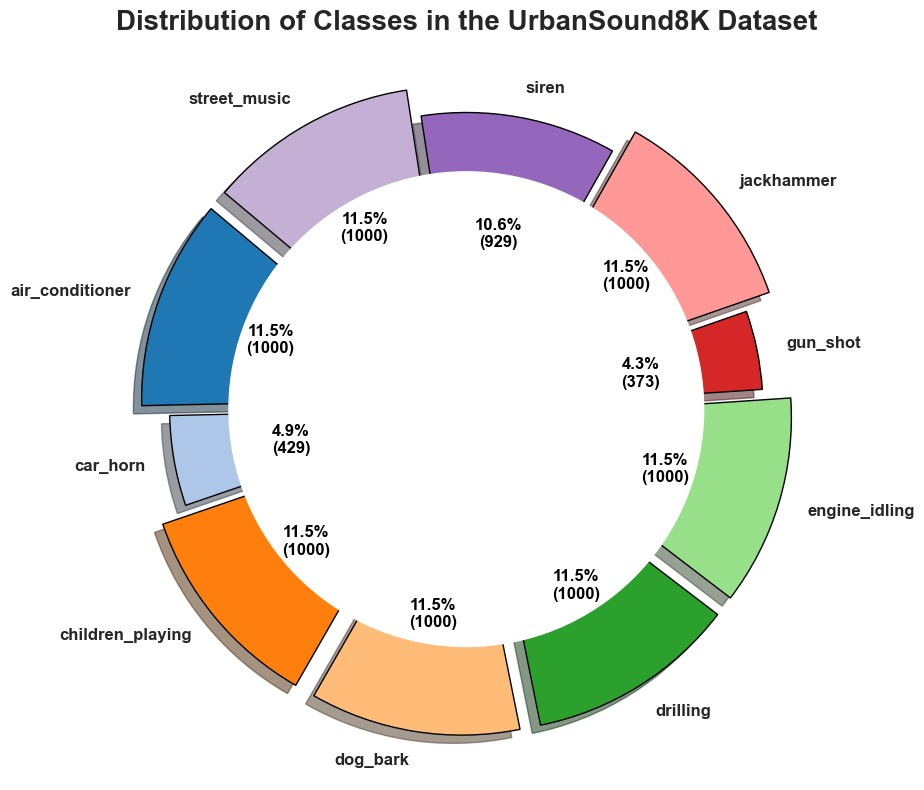
\includegraphics[width=0.45\textwidth]{Images/distribution.png}}
\caption{Distribution of noise types }
\label{fig:distribution}
\end{figure}


All excerpts in this data are taken from the "freesound" website, a repository of sound recordings. \cite{freesound}. Audio excerpt files are sorted into ten different folds in WAV format, these folders contain totally 8732 sound excerpts. Moreover, the data contains a CSV file containing metadata about each recording. The CSV file has meta-data information in 8 columns: the name of audio file, the freesound ID of the recording, the start time of the slice in the original recording, the end time of slice in the original recording, salience rating of the sound, the fold number, a numeric identifier of the sound class and the class name.

The sample rate, bit depth and number of channels are the same as the original file uploaded to Freesound. This ensures that the audio quality and characteristics remain consistent with the original recordings.



\begin{figure*}[htbp]
\centering
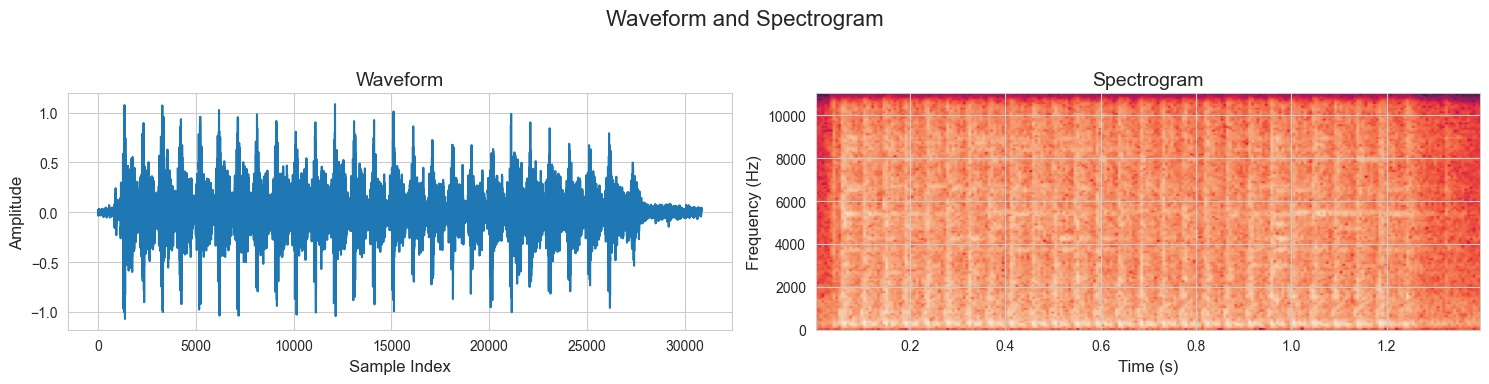
\includegraphics[width=\textwidth]{Images/signal.png}
\caption{Waveform and Spectrogram of an Urban Sound Clip}
\label{fig:waveform}
\end{figure*}

In Fig \ref{fig:waveform} illustrates a waveform and a spectrogram, two essential audio signal visualizations for comprehending various signal components.On the left side of the picture is the audio signal's waveform. A representation in the time domain is the waveform. It shows how the signal's amplitude varies with time. The sample index, which represents the discrete time points at which the audio signal was recorded, is represented on the x-axis. The amplitude or signal strength at each time point is shown by the y-axis. The waveforms peaks and troughs show how the audio signal loudness varies higher peaks correspond to louder sounds and deeper valleys to quieter times. The audio signal's spectrogram is displayed on the right side. A spectrogram is a time-frequency diagram that shows how the signal's frequency spectrum changes over time. In this case frequency is shown in hertz on the y-axis and time is represented in seconds on the x-axis. The color intensity at each point in the spectrogram indicates the magnitude of a certain frequency at a given time. Higher amplitudes and stronger frequency components are represented by brighter colors, whilst lower amplitudes and weaker frequency components are represented by less bright colors.Because it displays the precise frequency content of a signal across time, a spectrogram is an excellent tool for in-depth analysis of audio signals. The spectrogram offers information on how various frequencies vary and interact in a signal, in contrast to the waveform, which displays amplitude variations. This in-depth frequency domain data is crucial for tasks involving audio detection and classification, where a thorough understanding of the signal's properties is required. From the spectrogram, patterns, harmonic structures, and transient events can be seen that are difficult to see from the waveform by itself.

\begin{figure}[htbp]
\centerline{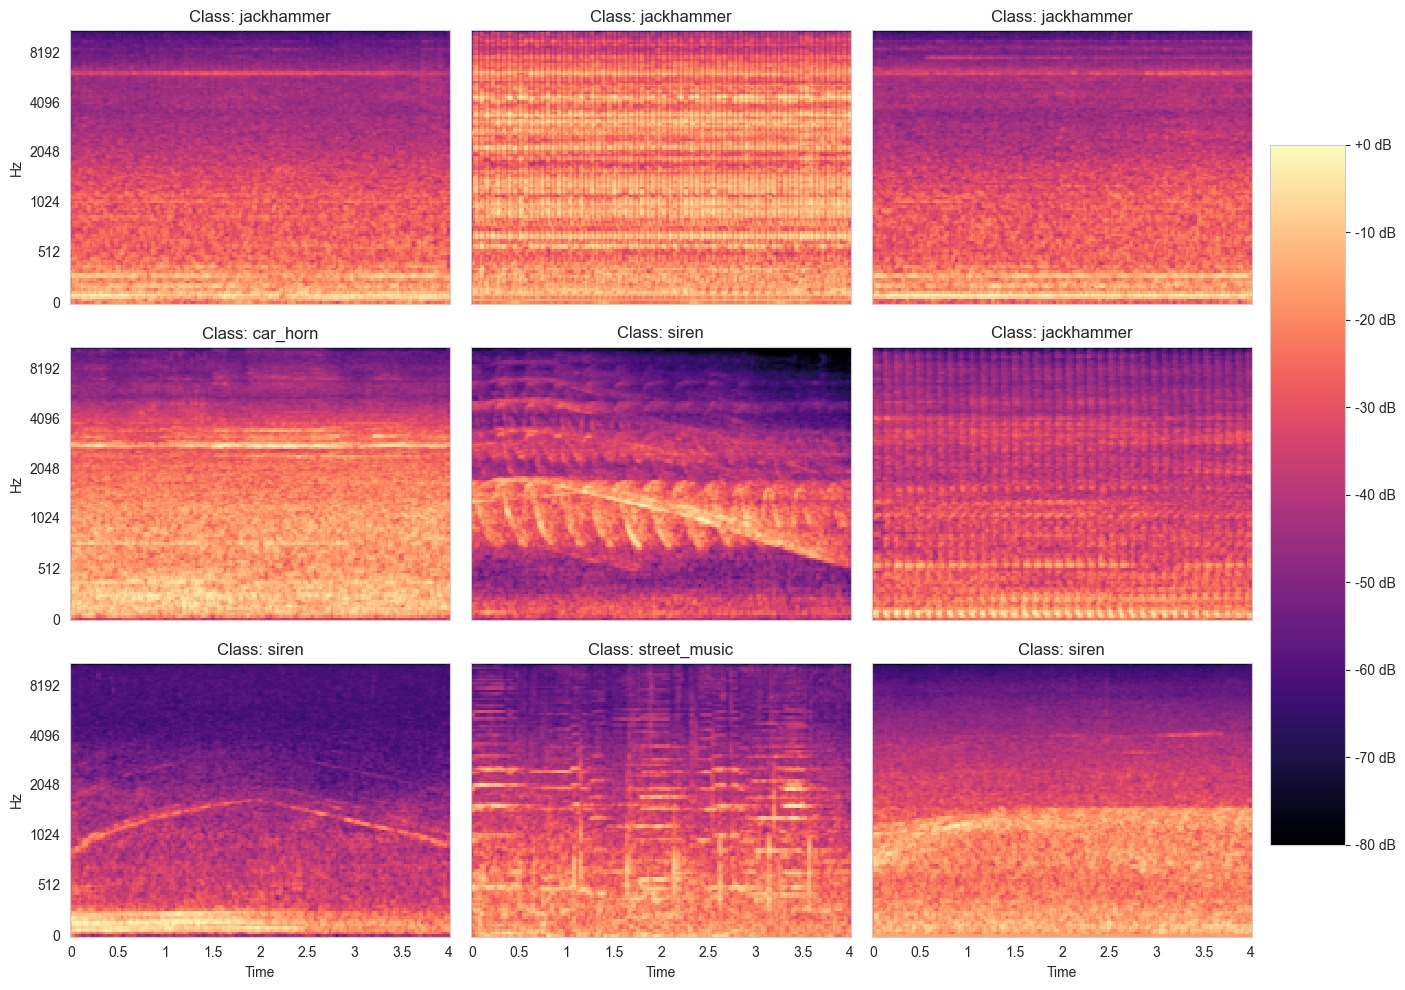
\includegraphics[width=0.5\textwidth]{Images/spectogram.png}}
\caption{Spectogram of noises }
\label{fig:spectogram}
\end{figure}


This is followed by a spectrogram of the identical sound signal that was acquired using the Librosa library in Fig \ref{fig:spectogram}. The color scale indicates the amplitude in decibels and the x- and y-axes display the time in seconds and the frequency in Hertz, respectively. A more thorough understanding of the frequency content over time is provided by this spectrogram, which also clearly demonstrates patterns for various sound classes. For example, sirens are represented by sweeping frequency patterns, car horns are sharp, noticeable lines at higher frequencies between 1000 and 6000 Hz, and street music is made up of more complex patterns over a wider frequency range. In order to precisely classify urban noises, a deep convolutional neural network must be trained with distinct acoustic characteristics for each class of sounds, as these visuals highlight. In order to build reliable and efficient models for the task of audio recognition, the waveform and spectrogram together provide complete insight into the temporal and spectral properties of the audio signals.



Through the usage of this dataset, models that can differentiate between different urban sound types can be developed for the purpose of classifying noise. In this study  this dataset is used  to develop artificial intelligence models that perform well in classifying various environmental noise types, so making a contribution to the larger field of urban sound analysis and classification.


\subsection{Algorithms}
In Fig 7 illustrates a waveform and a spectrogram, two es-
sential audio signal visualizations for comprehending various
signal components.On the left side of the picture is the audio
signal’s waveform. A representation in the time domain is the
waveform. It shows how the signal’s amplitude varies with
time. The sample index, which represents the discrete time
points at which the audio signal was recorded, is represented
on the x-axis. The amplitude, or signal strength at each time
point, is shown by the y-axis. The waveform’s peaks and
troughs show how the audio signal’s loudness varies; higher
peaks correspond to louder sounds and deeper valleys to
quieter times. The audio signal’s spectrogram is displayed
on the right side. A spectrogram is a time-frequency diagram
that shows how the signal’s frequency spectrum changes over
time. In this case, frequency is shown in hertz on the

\subsection{Code}

\subsubsection{Deep Neural Network (DNN)}
Deep Neural Networks' capacity to represent intricate patterns and relationships in data has allowed them to demonstrate outstanding performance in a number of domains, including picture and sound recognition. \cite{ca2023922991}Data preprocessing, model construction, training, and evaluation are some of the crucial stages that a DNN was used to do in order to classify urban sounds in the UrbanSound8K dataset.

\paragraph{Data Preprocessing}

The UrbanSound8K dataset, which includes audio clips from ten different classes, required features to be extracted in the first place. Mel-spectrogram coefficients were calculated in order to extract significant features from these audio files. These coefficients capture significant features that are more instructive for classification tasks and represent the sound's power spectrum.



\paragraph{Feature Extraction}

The audio clips were subjected to Mel-spectrogram feature extraction using the Librosa library. Mel-spectrograms convert time-domain signals into frequency domain signals and give an in-depth picture of the properties of the audio signal.\cite{inproceedings}


\paragraph{Normalization}
After that, the extracted features were normalized to ensure dataset consistency. Normalization plays a crucial role in accelerating the training process by preventing any one feature from outweighing the others in terms of helping the model learn.

\paragraph{Data Splitting}
The dataset was segregated into two parts: 80\% for training and the rest for testing. This split will allow the model to learn from a large amount of data, and its predictive prowess on unseen data will test its generalization capability.


\paragraph{Model Building}
The DNN's architecture was created using TensorFlow/Keras' Sequential API. The model is composed of multiple layers each of which plays a distinct role:



\begin{itemize}
    \item \textbf{Input Layer}: The input layer receives the preprocessed audio features, with the size of this layer corresponding to the number of features extracted from each audio clip.
    \begin{figure}[htbp]
\centerline{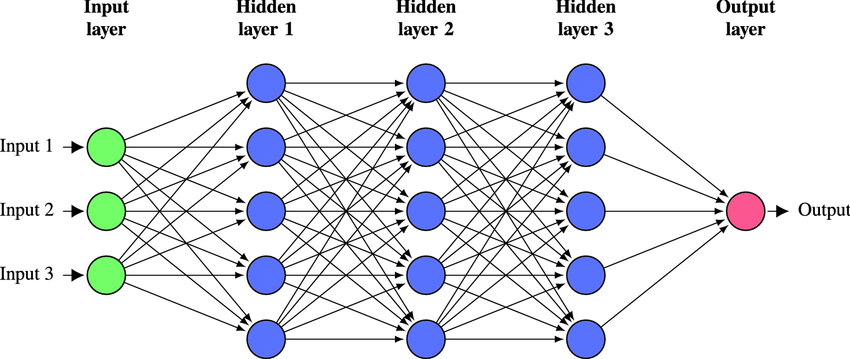
\includegraphics[width=0.5\textwidth]{Images/DNNsamplearchitect.png}}
\caption{A deep neural network (DNN) composed of an input layer of 3 nodes, 3 hidden layers of 5 nodes each, and an output layer of 1 node \cite{DNNsample}}
\label{fig:DNN Sample}
\end{figure}
    \item \textbf{Hidden Layers}: Several dense, or fully connected, layers with the ReLU activation function were employed. The non-linearity that ReLU offers enables the model to map more intricate patterns. To prevent overfitting, a dropout layer was added after every dense layer. In each training step dropout layers arbitrarily deactivate a portion of the neurons, forcing the network to acquire more robust features.

    
    \item \textbf{Output Layer}: Ten neurons, one for each of the ten classes, make up the output layer which has a softmax activation function. This makes the output applicable to multi-class classification tasks by enabling it to be converted into a probability distribution over the ten classes.

\end{itemize}

\paragraph{Training}
The Adam optimizer, a tried-and-true effective and flexible technique for training deep learning models, complied with the model. Sparse categorical cross-entropy, a suitable loss function for multi-class classification tasks, was used. A validation set comprising a portion of the training data was set aside to track the model's performance on unobserved data. It is trained with a batch size of 32 over 50 epochs.


\paragraph{Evaluation}
The test set is used to evaluate the model after it has been trained. A few metrics are used to assess the model's performance:


\begin{itemize}
    \item \textbf{Accuracy}:The primary metric indicating the proportion of correctly identified samples is 94.5\% indicating a respectable accuracy of the DNN with regard to the test set.

    \item \textbf{Precision, Recall, and F1-Score}: These metrics offer a thorough assessment of the model's effectiveness in various courses. The percentage of true positive forecasts among all positive predictions is known as precision. Recall compares all real positives to the percentage of genuine positive forecasts. The harmonic mean of recall and accuracy is thus the F1-score.
    
\begin{table}[htbp]
\centering
\begin{tabular}{lcccc}
\toprule
 & \textbf{Precision} & \textbf{Recall} & \textbf{F1-Score} & \textbf{Support} \\
\midrule
\textbf{Class 0} & 0.98 & 0.99 & 0.98 & 250 \\
\textbf{Class 1} & 0.96 & 0.93 & 0.95 & 107 \\
\textbf{Class 2} & 0.90 & 0.96 & 0.92 & 250 \\
\textbf{Class 3} & 0.90 & 0.89 & 0.90 & 250 \\
\textbf{Class 4} & 0.96 & 0.93 & 0.95 & 250 \\
\textbf{Class 5} & 0.98 & 1.00 & 0.99 & 250 \\
\textbf{Class 6} & 0.94 & 0.82 & 0.88 & 94 \\
\textbf{Class 7} & 0.95 & 0.98 & 0.97 & 250 \\
\textbf{Class 8} & 0.97 & 0.97 & 0.97 & 232 \\
\textbf{Class 9} & 0.92 & 0.91 & 0.91 & 250 \\
\midrule
\textbf{Accuracy} &  &  & 0.95 & 2183 \\
\textbf{Macro avg} & 0.95 & 0.94 & 0.94 & 2183 \\
\textbf{Weighted avg} & 0.95 & 0.95 & 0.95 & 2183 \\
\bottomrule
\end{tabular}
\caption{DNN Precision, Recall, and F1-Score Table }
\label{tab:classification_report}
\end{table}
    \item \textbf{Confusion Matrix}: A confusion matrix was generated to visualize the model's performance across different classes showing the number of correct and incorrect predictions for each class.
\begin{figure}[htbp]
\centerline{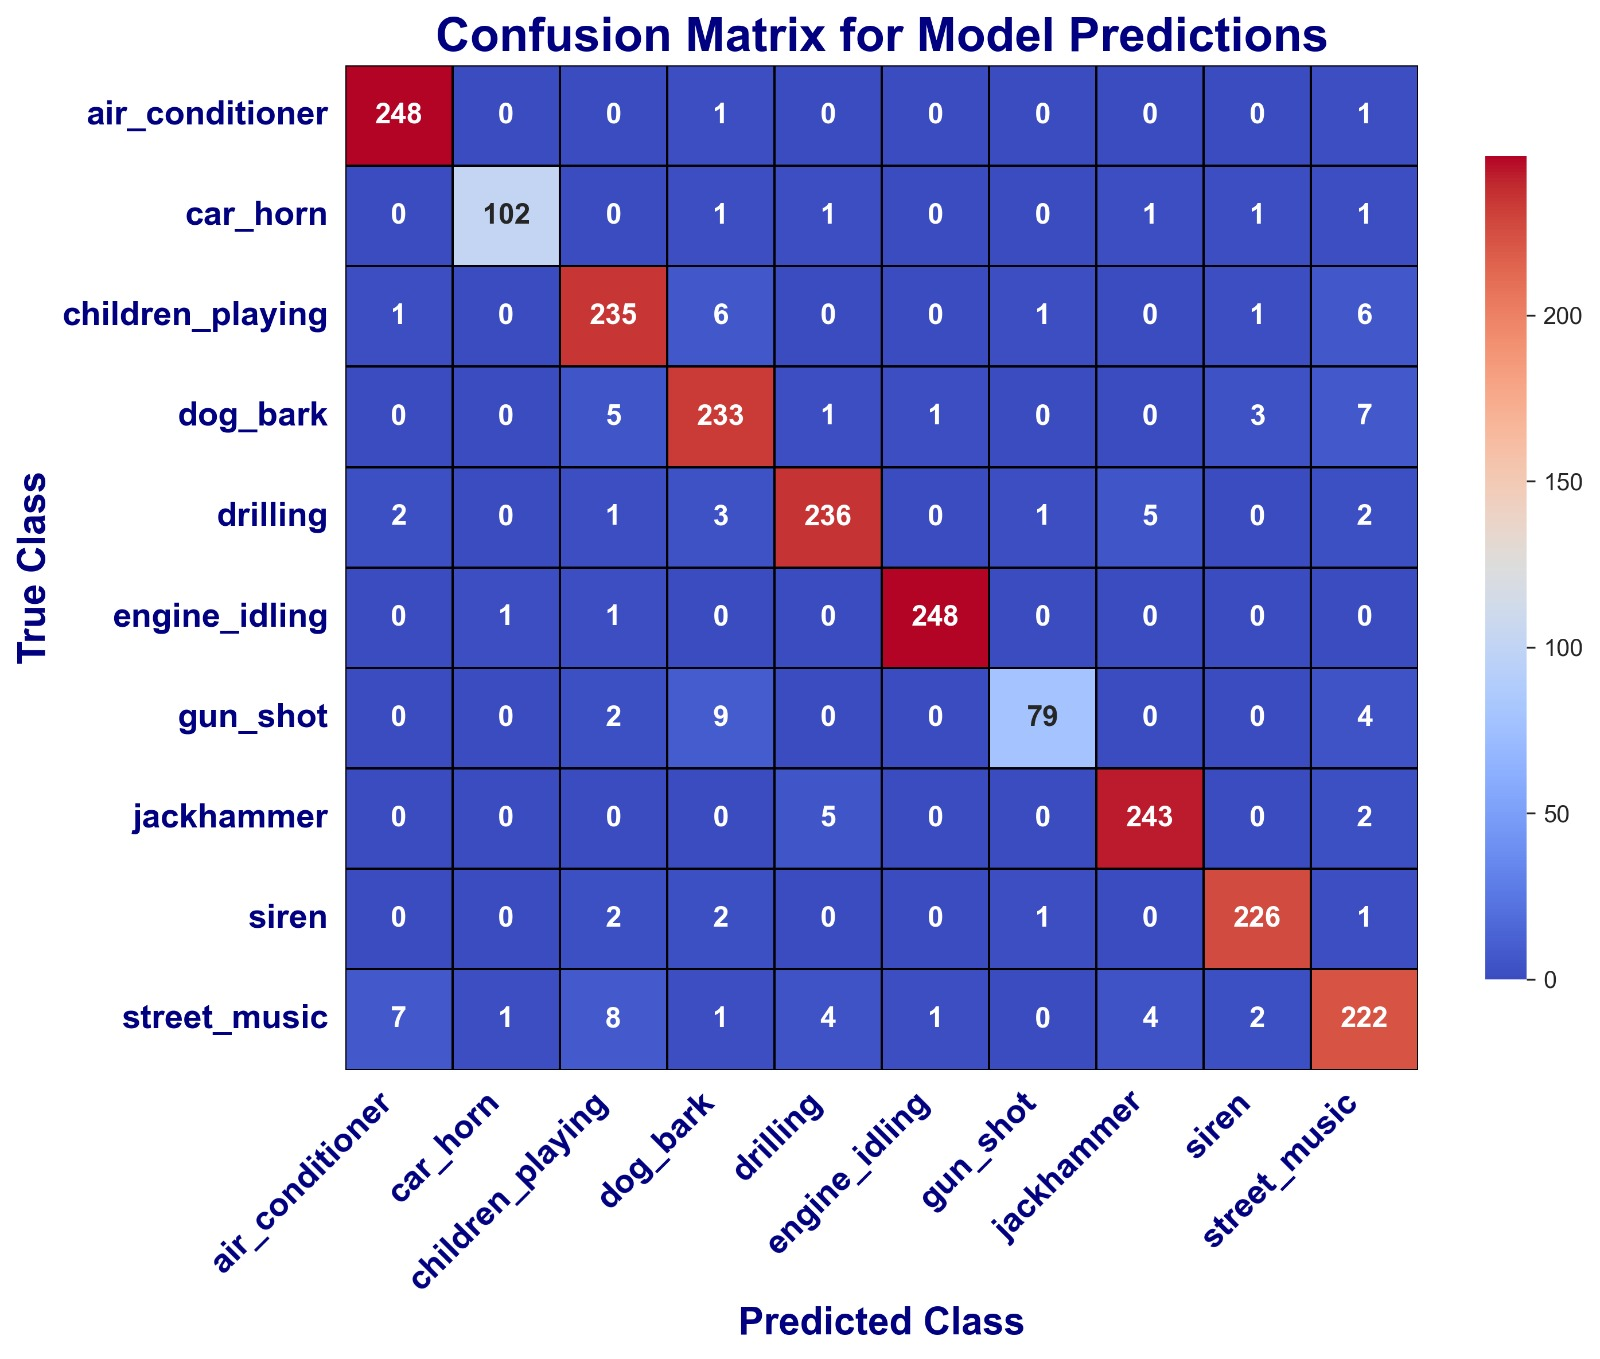
\includegraphics[width=0.5\textwidth]{Images/DNNconfusion.png}}
\caption{DNN Confusion Matrix}
\label{fig:DNNconfusion}
\end{figure}
\end{itemize}


\begin{figure}[htbp]
\centerline{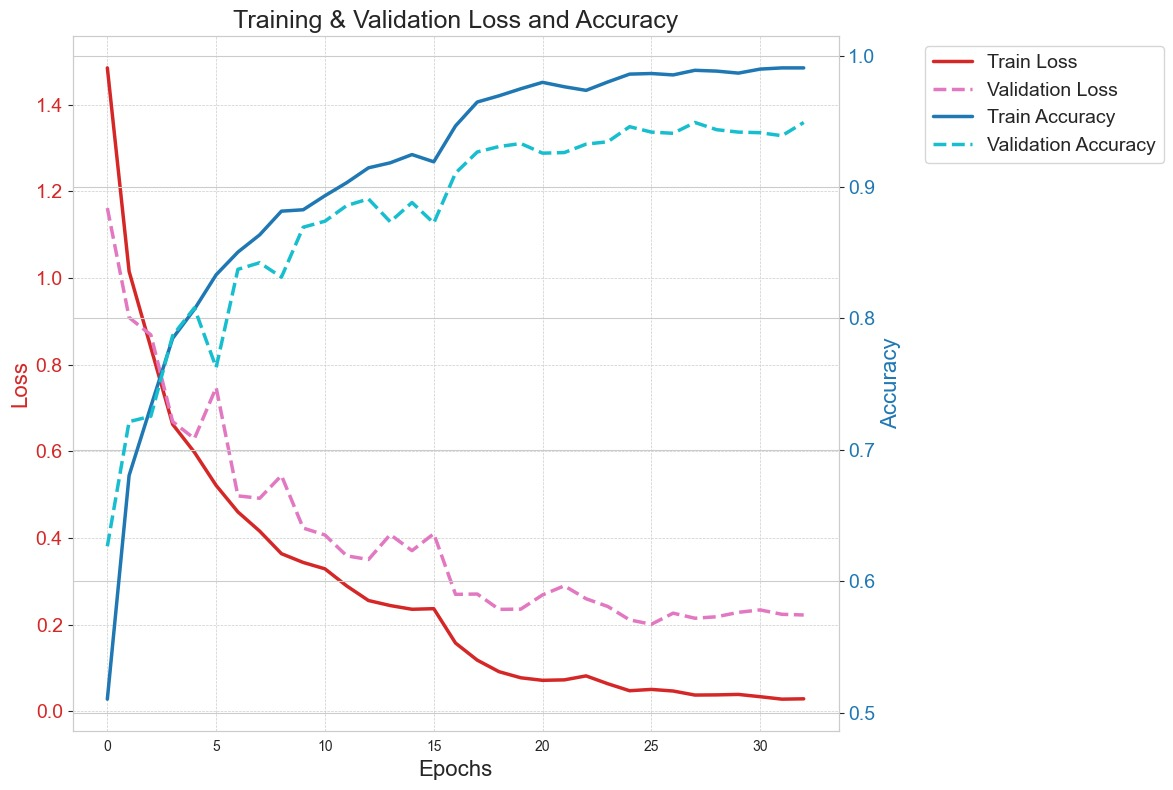
\includegraphics[width=0.5\textwidth]{Images/DNNgraph.png}}
\caption{DNN}
\label{fig:DNNgraph}
\end{figure}



\paragraph{}{Results and Discussion}
The DNN model's high accuracy shows how well it can identify and understand intricate patterns in audio data. There are several reasons for the model's success:


\begin{itemize}
    \item \textbf{Hierarchical Learning:} In other words, the DNN learns to represent the input characteristics in a hierarchical fashion, storing high-level, abstract information in the deeper layers and low-level data in the lower levels.

    \item \textbf{Regularization:}By adding dropout layers, they were able to prevent overfitting and enable the model to generalize to new data.

    \item \textbf{Optimization:} The model's training and convergence were facilitated by the Adam optimizer's flexible learning rate.

\end{itemize}

\subsubsection{Random Forest}
An UrbanSound8K dataset including 8732 audio clips of 10 urban sound classes—such as sirens, dog barking, and automobile horns—will be the source of data for this study. These audio files' metadata is loaded, containing details like the file name, fold number, and class label.


The preprocessing phase involves several crucial tasks:

\paragraph{Feature Extraction}
One important step in converting unprocessed audio data into a set of representative characteristics that the Random Forest classifier will employ is feature extraction. In response, a variety of audio-related properties are retrieved.

\begin{itemize}
    \item \textbf{Mel-frequency Cepstral Coefficients (MFCCs)}: The description of the timbre texture is one of the primary applications of the MFCCs in speech and audio processing, which are used to record the power spectrum of the audio input.

    \item \textbf{Chroma Features}: These characteristics are helpful in capturing the harmonic content and the energy distribution among the twelve pitch classes.


    \item \textbf{Spectral Contrast}: This function assists in differentiating between harmonic and noisy sounds by calculating the amplitude difference between peaks and troughs in the sound spectrum.

\end{itemize}

To lower the dataset's dimensionality and provide a fixed-size feature vector for every audio recording, extracted features are averaged over time. By removing less significant temporal irregularities, this averaging aids in preserving the main qualities of the audio input.


\paragraph{Data Splitting and Label Encoding}

The dataset may be split into training and testing groups once features are extracted. In order to get a nearly similar class balance in each subset, this is often done in a stratified manner. This is crucial for training a balanced model. Typically, 20\% is set up for testing and 80% for instruction.


Next, the class of each audio file is mapped onto a number value using label encoding. Numerical input is required for machine learning models, which makes this method vital. The random forest classifier then uses the encoded labels to analyze and process category input.


\paragraph{Building and Training the Random Forest Model}

Using a large number of decision trees, the Random Forest ensemble learning technique aims to increase resilience and accuracy. The steps involved in implementing Random Forest are listed below:


\begin{itemize}
    \item \textbf{Initialization}: The Random Forest model is initialized with a specified number of trees (\textit{n\_estimators}). In this study, 100 trees were used, which is a common choice that balances performance and computational cost.
    \item \textbf{Training}: Next, the training set is fitted to the model. A random subset of characteristics is considered at each node in the forest when constructing each tree by taking a bootstrap sample of the data. The model's predictive power is enhanced and overfitting is reduced by this unpredictability.

    \item \textbf{Aggregation}: For classification jobs, majority voting is used to aggregate all of the aforementioned tree forecasts. Collectively, these trees' strengths are maximized while their flaws are mitigated.

\end{itemize}

\paragraph{}{Model Evaluation}

The performance of the trained Random Forest model is evaluated on the test set using several metrics:

\begin{itemize}
    \item \textbf{Accuracy}: This score assesses how accurate the model's predictions are overall. The ratio of correctly categorized instances to the total number of instances is used to determine it.

    \item \textbf{Precision, Recall, and F1-Score}: These metrics offer a more thorough assessment of the model's performance in each of the classes. The F1 score is the harmonic mean of accuracy and recall. accuracy may be used to determine what percentage of the positive predictions were really positive. Recall can be used to determine what percentage of the actual positives were anticipated favorably.


    \item \textbf{Confusion Matrix}: A confusion matrix is made to show how well the model performs in various classes. It makes clear which forecasts are accurate and which are inaccurate for every class, making it possible to pinpoint the precise areas in the model that require improvement.

\end{itemize}

\paragraph{Summary}

In order to guarantee the accuracy and dependability of the model, there are several crucial phases involved in implementing the Random Forest classifier for urban noise categorization. The loading and preparation of the UrbanSound8K dataset is the first step in the process, after which significant audio characteristics are extracted. After the labels are encoded into numerical values, the data is divided into training and testing subsets.

Multiple decision trees are joined to increase performance during the building and training of the Random Forest model, which is done using an ensemble technique. The trained model's accuracy in classifying urban sounds is comprehensively assessed through the use of many criteria.

This thorough implementation emphasizes the significance of every stage involved and shows how well the Random Forest classifier handles the challenging urban noise categorization tasks. The outcomes highlight the model's dependability and possible uses in urban sound monitoring and categorization systems in the actual world.



\begin{table}[htbp]
\centering
\begin{tabular}{lcccc}
\toprule
 & \textbf{Precision} & \textbf{Recall} & \textbf{F1-Score} & \textbf{Support} \\
\midrule
\textbf{Class 0} & 0.86 & 0.94 & 0.90 & 203 \\
\textbf{Class 1} & 1.00 & 0.69 & 0.81 & 86 \\
\textbf{Class 2} & 0.72 & 0.80 & 0.76 & 183 \\
\textbf{Class 3} & 0.89 & 0.87 & 0.88 & 201 \\
\textbf{Class 4} & 0.86 & 0.86 & 0.86 & 206 \\
\textbf{Class 5} & 0.95 & 0.97 & 0.96 & 193 \\
\textbf{Class 6} & 0.89 & 0.76 & 0.81 & 72 \\
\textbf{Class 7} & 0.93 & 0.91 & 0.92 & 208 \\
\textbf{Class 8} & 0.89 & 0.93 & 0.91 & 205 \\
\textbf{Class 9} & 0.80 & 0.76 & 0.78 & 230 \\
\midrule
\textbf{Accuracy} &  &  & 0.87 & 1747 \\
\textbf{Macro avg} & 0.85 & 0.84 & 0.85 & 1747 \\
\textbf{Weighted avg} & 0.87 & 0.87 & 0.87 & 1747 \\
\bottomrule
\end{tabular}
\caption{Random Forest Classification Report}
\label{tab:classification_report}
\end{table}


\begin{figure}[htbp]
\centerline{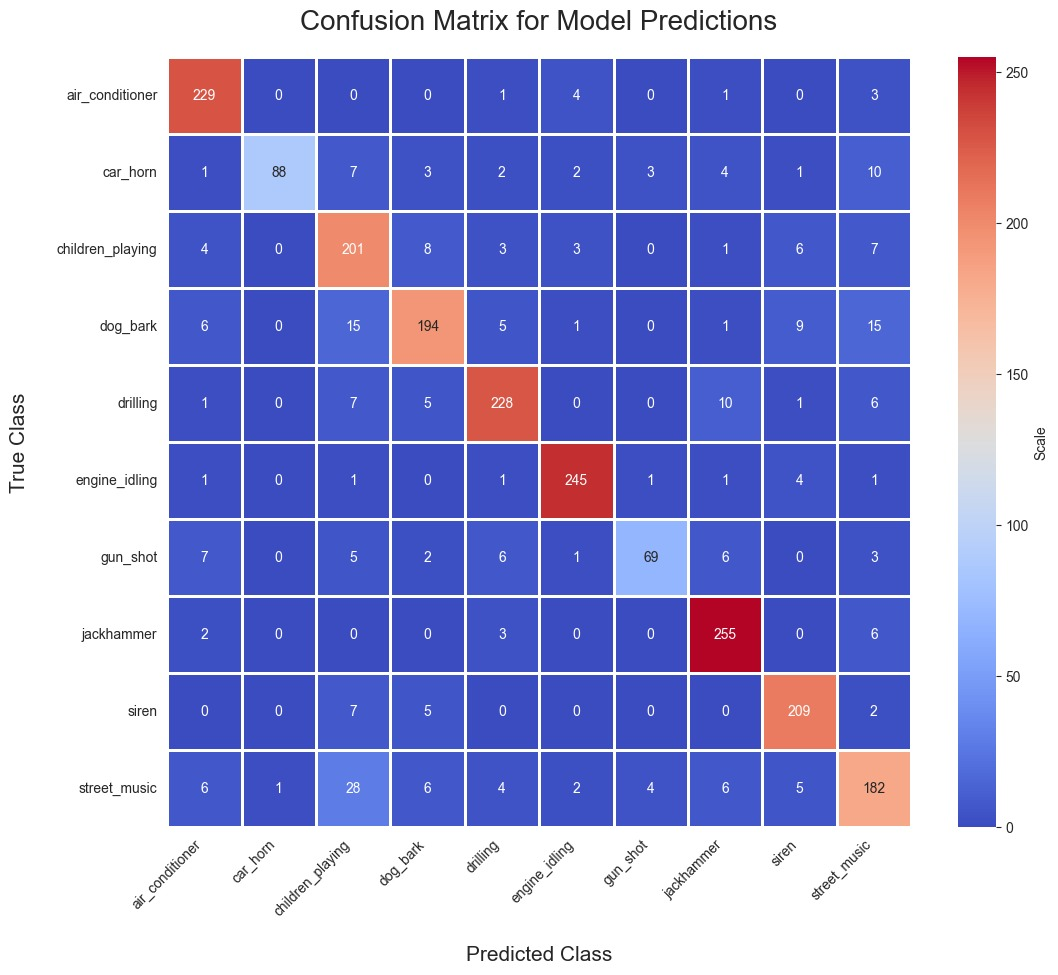
\includegraphics[width=0.5\textwidth]{Images/RFgraph.png}}
\caption{Random Forest Confusion Matrix}
\label{fig:RFconfusion}
\end{figure}

\subsubsection{Long Short Term Memory (LSTM)}
The Long Short-Term Memory network's implementation details for the task of identifying urban sounds using the UrbanSound8K dataset are covered in this section. Because it can capture the temporal patterns and long-term relationships present in audio signals, the LSTM network is a good fit for this purpose.


The sequential structure of the audio data makes the LSTM model well-suited to learn from it. An LSTM model's architecture may include one or more of the following elements:


\paragraph{Input Layer}
The audio's preprocessed characteristics at the input layer are: The audio's features—that is, samples, time steps, and features—are transformed into three dimensions since LSTMs need three-dimensional input. To make sure the model can handle every feature in incremental steps, it is being reshaped.


\paragraph{LSTM Layers}
The temporal dependencies of the audio data are captured by the LSTM layers that make up the core. The following are included in the model:

\begin{itemize}
    \item \textbf{First LSTM Layer}: In addition to having 128 units, the layer is configured to return sequences. Sequences that are returned enable the next LSTM layer to process the whole data sequence.


    \item \textbf{Second LSTM Layer}: The last output in the series is what this 64-unit layer is supposed to return. This arrangement aids in dimensionality reduction while preserving temporal information discovered in the layer before.

\end{itemize}

\paragraph{Dropout Layers}
To prevent overfitting, a dropout layer is inserted after every LSTM layer. Randomly set to zero is a portion of the input units during training. One of the regularizations used to make sure the model can more broadly apply to unknown data is to prevent it from being overly reliant on a particular neuron.


\paragraph{Fully Connected Layers}
The dense layers, which are totally linked, appear after the LSTM layers. These tiers aid in the categorization step and aid in the subsequent processing of the learnt information.

\begin{itemize}
    \item \textbf{First Dense Layer}: There are thirty-two units with ReLU activation functions in this layer. ReLU gives the model non-linearity, which enables it to learn intricate patterns.

    \item \textbf{Output Layer}: Ten units, or the number of sound classes, with a softmax activation function are included in this layer. Because the softmax function offers probabilities across classes, it may be used to solve multi-class classification issues.

\end{itemize}

The following setup is used to compile and train the model:


\paragraph{Loss Function}
Categorical cross-entropy serves as the loss function and is useful in multi-class classification. This function guides the optimization process by measuring the discrepancy between the true class labels and the anticipated probability.

\paragraph{Optimizer}
Since the Adam optimizer is effective and well-suited to managing sparse gradients, we have chosen it. The estimated first and second moments of the gradient are used to modify the learning rate.


\paragraph{Metrics}
The main statistic used to assess the model's performance during training and testing is accuracy. The percentage of properly identified samples relative to all samples is known as accuracy.

\paragraph{Training Process}
The model is trained with a batch size of 32 across many epochs. In order to improve training efficiency and avoid overfitting, countermeasures such as early halting and learning rate decrease on plateau are used. While learning rate reduction lowers the learning rate when the validation loss reaches a plateau, early stopping tracks the validation loss and ends training when it stops getting better.

The performance of the trained LSTM model is assessed using the test set. Various important measures are employed:


\paragraph{Accuracy}
The degree to which the model can accurately categorize the urban sound snippets is shown by the model's overall accuracy on the test set.


\begin{figure}[htbp]
\centerline{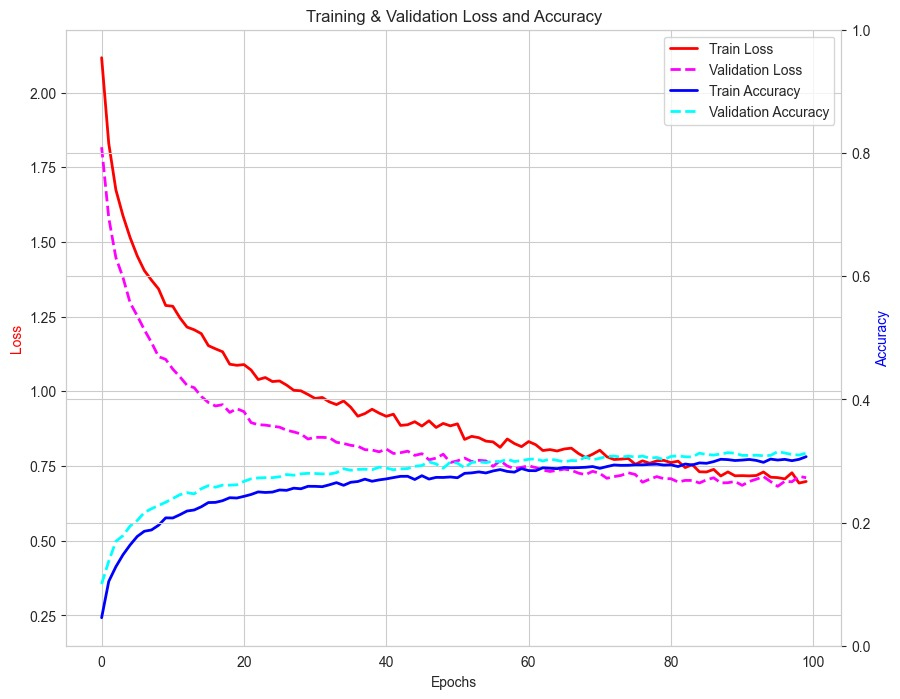
\includegraphics[width=0.5\textwidth]{Images/LSTMgraph.png}}
\caption{LSTM Graph}
\label{fig:LSTMgraph}
\end{figure}

\paragraph{Confusion Matrix}
To give a thorough analysis of the model's performance across the various sound classes, a confusion matrix is created. The number of accurate and inaccurate predictions for each class is displayed in this matrix, providing information about the model's advantages and disadvantages.


\begin{figure}[htbp]
\centerline{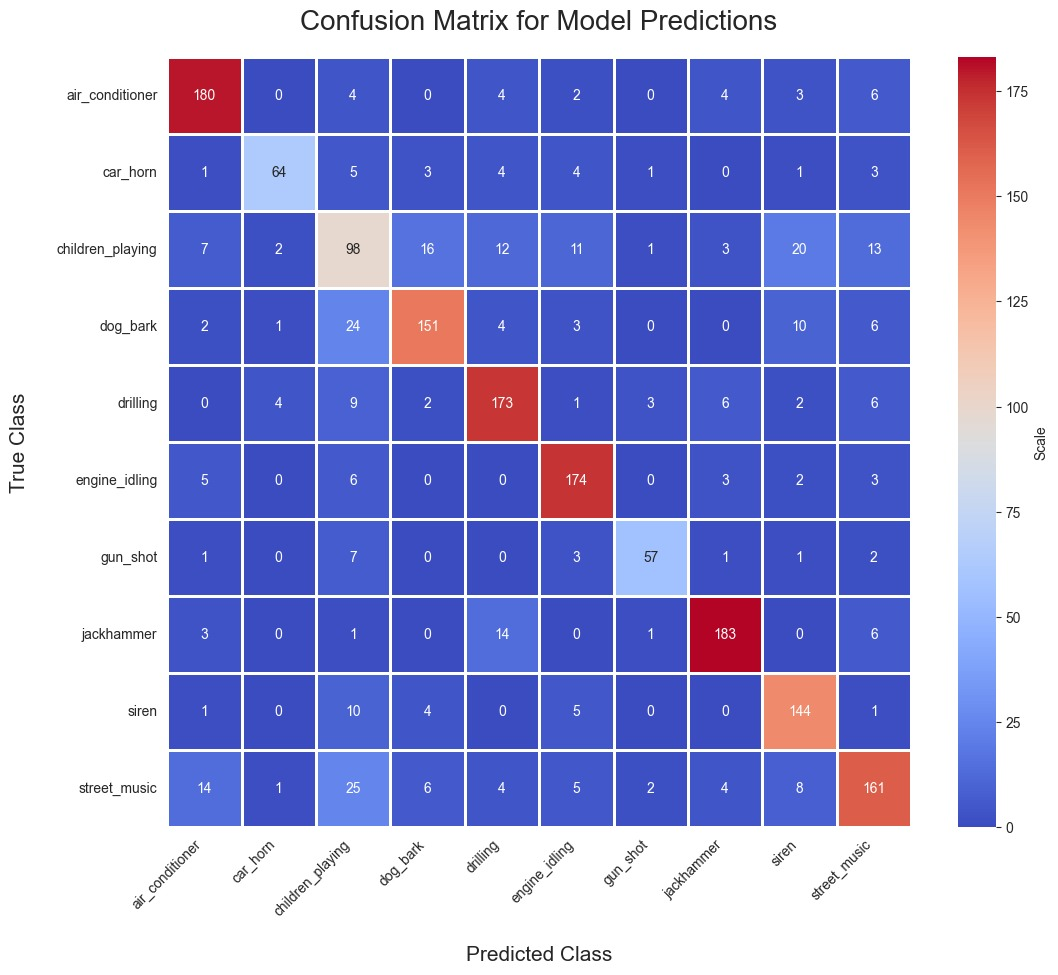
\includegraphics[width=0.5\textwidth]{Images/LSTMconfusion.png}}
\caption{LSTM Confusion Matrix}
\label{fig:LSTMconfusion}
\end{figure}

\paragraph{Precision, Recall, and F1-Score}
For every class, these metrics are computed to evaluate the model's accuracy, recall, and balance (F1-score) between capturing all relevant examples and accurately identifying positive occurrences.

The capacity of the LSTM model to recognize and learn from the temporal patterns in audio data is demonstrated by its application to the categorization of urban sounds. The architecture of the model takes use of the sequential nature of the input characteristics by arranging numerous LSTM layers in front of dense layers. The model delivers effective classification performance through the use of strong training and assessment methodologies, as demonstrated by the confusion matrix and other evaluation metrics as well as the model's accuracy and extensive analysis. The capabilities of LSTM networks in audio identification tasks, especially in intricate and dynamic metropolitan situations, are demonstrated by this application.

\subsubsection{Convolutional Neural Networks (CNN)}

The spectrograms of the audio data's spatial hierarchy are a valuable source of learning information for the CNN model.\cite{improve}The CNN model's architecture consists of the following elements:


\paragraph{Input Layer}
The input layer receives the preprocessed spectrogram features. Given that CNNs require three-dimensional input (samples, height, width, and channels), the spectrogram features are reshaped accordingly.

\paragraph{Convolutional Layers}
The core of the model consists of convolutional layers. These layers are responsible for detecting local patterns and features in the spectrograms. The model includes:
\begin{itemize}
    \item \textbf{First Convolutional Layer}: This layer consists of 32 filters with a kernel size of 3x3 and a ReLU activation function. It captures low-level features such as edges.
    \item \textbf{Pooling Layer}: A max-pooling layer with a pool size of 2x2 is applied to reduce the dimensionality and retain the most important features.
    \item \textbf{Second Convolutional Layer}: This layer consists of 64 filters with a kernel size of 3x3 and a ReLU activation function. It captures more complex patterns.
    \item \textbf{Pooling Layer}: Another max-pooling layer with a pool size of 2x2 is applied to further reduce dimensionality.
\end{itemize}

\paragraph{Dropout Layers}
Dropout layers are incorporated after each pooling layer to prevent overfitting by randomly setting a fraction of input units to zero during training. This regularization technique helps in ensuring that the model does not become too dependent on specific neurons and can generalize better to unseen data.

\paragraph{Fully Connected Layers}
Following the convolutional layers, the model includes dense (fully connected) layers. These layers further process the learned features and aid in classification.
\begin{itemize}
    \item \textbf{First Dense Layer}: This layer consists of 128 units with a Rectified Linear Unit (ReLU) activation function. ReLU introduces non-linearity into the model enabling it to learn complex patterns.
    \item \textbf{Output Layer}: This layer consists of 10 units, corresponding to the ten sound classes, with a softmax activation function. The softmax function outputs probability distributions over the classes, making it suitable for multi-class classification tasks.
\end{itemize}

The model is compiled and trained using the following configurations:

\paragraph{Loss Function}
Categorical cross-entropy is used as the loss function, appropriate for multi-class classification tasks. This function measures the difference between the true class labels and the predicted probabilities, guiding the optimization process.

\paragraph{Optimizer}
The Adam optimizer is selected for its efficiency and capability to handle sparse gradients. Adam adjusts the learning rate dynamically based on the first and second moments of the gradient, ensuring faster convergence.

\paragraph{Metrics}
Accuracy is used as the primary metric to evaluate the model's performance during training and testing. Accuracy measures the proportion of correctly classified samples out of the total samples.

\paragraph{Training Process}
The model is trained over multiple epochs with a batch size of 32. Early stopping and learning rate reduction on plateau are employed as callbacks to enhance training efficiency and prevent overfitting. Early stopping monitors the validation loss and stops training when it stops improving, while learning rate reduction reduces the learning rate when the validation loss plateaus.

The trained CNN model is evaluated on the test set to measure its performance. Several key metrics are used:

\paragraph{Accuracy}
The overall accuracy of the model on the test set provides a measure of how well the model can correctly classify the urban sound excerpts.

\begin{figure}[htbp]
\centerline{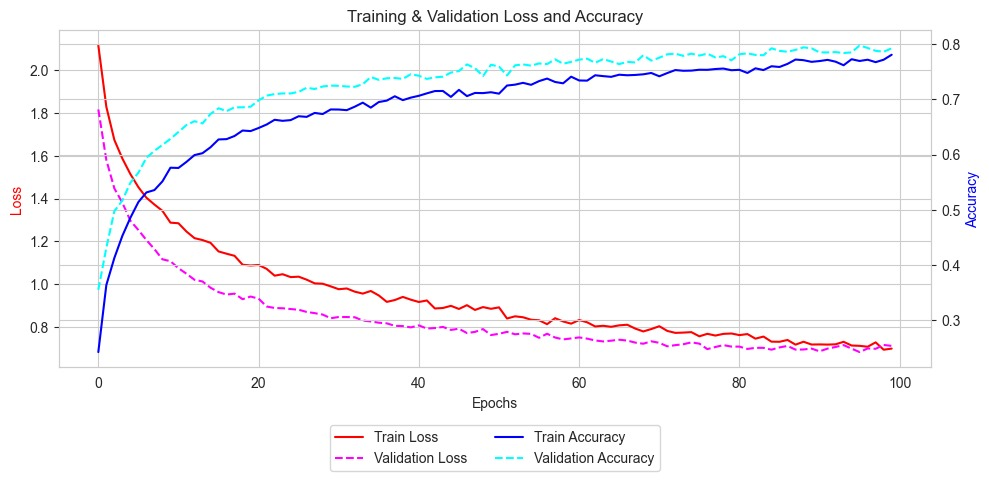
\includegraphics[width=0.5\textwidth]{Images/CNNgraph.png}}
\caption{CNN Graph}
\label{fig:LSTMconfusion}
\end{figure}


\paragraph{Confusion Matrix}
A confusion matrix is generated to provide a detailed breakdown of the model's performance across the different sound classes. This matrix highlights the number of correct and incorrect predictions for each class, offering insights into the model's strengths and areas for improvement.

\begin{figure}[htbp]
\centerline{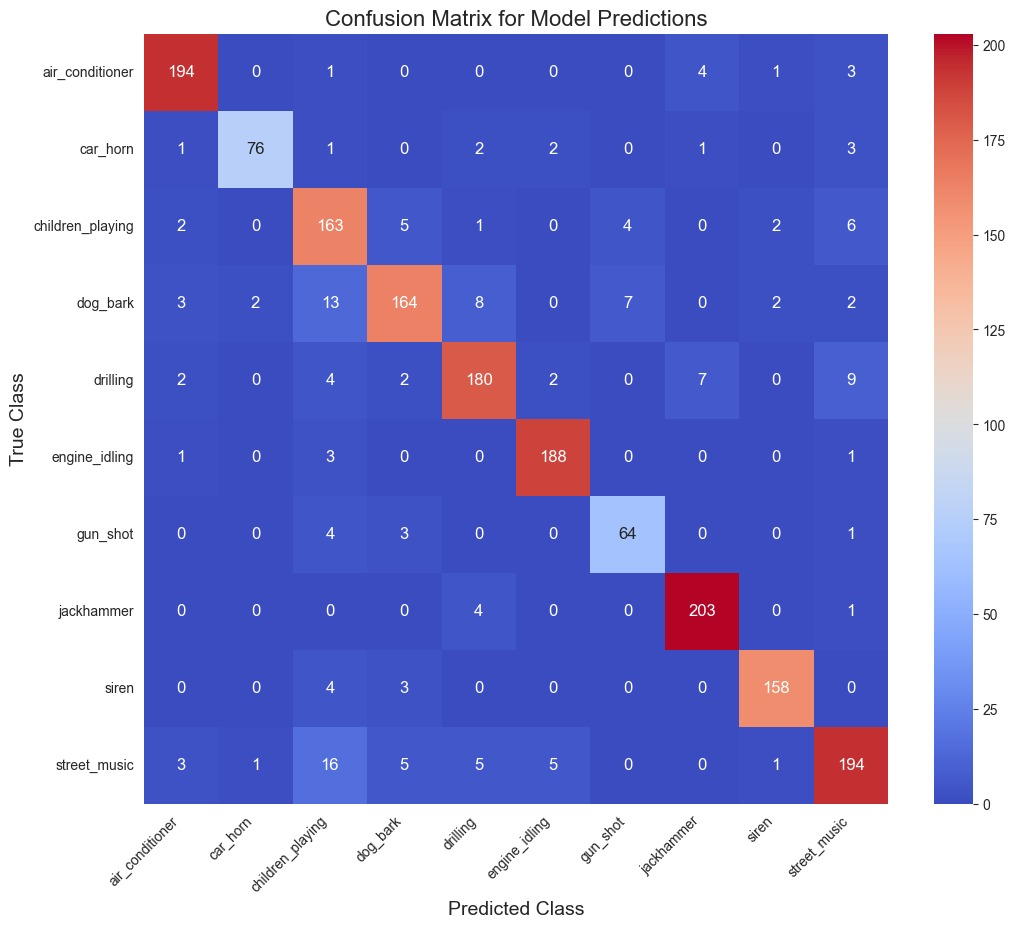
\includegraphics[width=0.5\textwidth]{Images/CNNconfusion.png}}
\caption{CNN Confusion Matrix}
\label{fig:LSTMconfusion}
\end{figure}

\paragraph{Precision, Recall, and F1-Score}
These metrics are calculated for each class to assess the model's ability to correctly identify positive instances (precision), its ability to capture all relevant instances (recall), and the balance between precision and recall (F1-score).

The CNN model's capacity to recognize and learn from the spatial hierarchies in the spectrogram data is demonstrated by its application to the categorization of urban sounds.\cite{Sharma} The architecture of the model makes use of the local patterns and characteristics seen in the spectrograms. It consists of many convolutional layers followed by dense layers. The model delivers effective classification performance through the use of strong training and assessment methodologies, as demonstrated by the confusion matrix and other evaluation metrics as well as the model's accuracy and extensive analysis. This implementation demonstrates CNNs' promise for audio identification tasks, especially in intricate and dynamic metropolitan settings.


\begin{table}[ht]
    \centering
    \begin{tabular}{lcccc}
        \hline
        Class & Precision & Recall & F1-score & Support \\
        \hline
        air\_conditioner & 0.94 & 0.96 & 0.95 & 203 \\
        car\_horn & 0.95 & 0.84 & 0.89 & 86 \\
        children\_playing & 0.75 & 0.86 & 0.80 & 183 \\
        dog\_bark & 0.89 & 0.86 & 0.87  & 201 \\
        drilling & 0.92 & 0.84 & 0.88 & 206 \\
        engine\_idling & 0.93 & 0.96 & 0.95 & 193 \\
        gun\_shot & 0.87 & 0.85 & 0.86 & 72 \\
        jackhammer & 0.97 & 0.96 & 0.96 & 208 \\
        siren & 0.87 & 0.97 & 0.92 & 165 \\
        street\_music & 0.88 & 0.81 & 0.84 & 230 \\
        \hline
        accuracy & \multicolumn{4}{c}{0.89 (1747)} \\
        macro avg & 0.90 & 0.89 & 0.89 & 1747 \\
        weighted avg & 0.90 & 0.89 & 0.89 & 1747 \\
        \hline
    \end{tabular}
        \caption{Classification Report for CNN}
    \label{tab:classification_repor}
\end{table}



\subsection{System Settings}
The underlying software and hardware settings have a significant impact on the repeatability and performance of machine learning studies. Thorough explanations of the system configurations guarantee consistent outcomes and offer background information for any performance measurements that are disclosed. Every experiment was carried out on a device that met the following requirements:

\begin{itemize}
    \item \textbf{Processor:} Intel Core i7-13650HX (20 CPUs) @ 2.60GHz
    \item \textbf{Memory:} 16 GB RAM
    \item \textbf{Graphics:} NVIDIA GeForce RTX 4060
    \item \textbf{Operating System:} Windows 11
    \item \textbf{Storage:} 1 TB SSD
\end{itemize}

The software environment was configured as follows:
\begin{itemize}
    \item \textbf{Python Version:} 3.11.9
    \item \textbf{Libraries:}
    \begin{itemize}
        \item \texttt{librosa} - 0.10.2.post1
        \item \texttt{numpy} - 1.26.4
        \item \texttt{pandas} - 2.2.2
        \item \texttt{scikit-learn} - 1.4.2
        \item \texttt{seaborn} - 0.13.2
        \item \texttt{matplotlib} - 3.9.0
        \item \texttt{tensorflow} - 2.16.1
        \item \texttt{keras} - 3.3.3
        \item \texttt{warnings} (part of the Python standard library)
    \end{itemize}
    \item \textbf{IDE:} Visual Studio Code
\end{itemize}


\section{Future Directions}
There are numerous areas where machine learning for the classification of urban noise can be further explored, with the goal of improving the practicality, effectiveness, and resilience of existing approaches. The first is about sound event detection automation. Currently, segmenting a continuous stream of sounds involves numerous manual steps. The creation of completely automated SED systems would significantly increase the scalability and efficiency of applications used in the classification of urban noise.\cite{tsalera2020monitoring}\cite{kim2021data} Modern machine learning techniques, particularly deep learning models, can be used by Automatic SED to precisely detect and segment sound events in real-time with less need for human interaction, increasing system accuracy.

The optimization of the feature selection and extraction procedures is a crucial area that requires additional effort. Reducing the amount of parameters used in categorization is necessary since IoT sensors and other equipment used for monitoring urban noise often have limited processing capabilities.\cite{8300941}\cite{alsouda2018machine}  In addition to reducing the computational burden, feature reduction makes sure that the characteristics chosen are actually useful to enhancing the classification models' accuracy. Subsequent investigations ought to concentrate on pinpointing the most crucial features and exploring methods for achieving feature optimization via dimensionality reduction, feature engineering, and the application of sophisticated algorithms like as PCA and t-SNE.\cite{8300941}

Furthermore, even more complex neural network architectures, such as long short-term memory networks and convolutional neural networks, will be incorporated to improve the performance of the urban noise categorization models.\cite{tsalera2020monitoring} Because these structures can capture the temporal and spatial connections in the data, they are highly suited for processing audio data. Therefore, future models can categorize the complex and overlapping sound events that are typical in urban areas with more accuracy by utilizing CNNs and LSTMs.

Moreover, another area where further effort should be done is the deployment of advanced models onto edge devices.\cite{tsalera2020monitoring} By allowing real-time noise categorization to be performed directly on the devices from which the data was collected, edge computing might potentially reduce response time and latency. Thus, it is necessary to create compact, effective models that can operate on the limited resources that edge devices provide while yet achieving good classification performance.

Finally, in order to support the dataset's diversification and enlarge it, new cooperative and crowdsourced methods of data collection need to be investigated. By including the community in the data gathering process, the researchers will be able to obtain a representative sample of urban noises that will enable the creation of more robust and generalized categorization models.\cite{mishachandar2021diverse} It will be equally crucial to put privacy-preserving measures into practice to guarantee the moral use of the information gathered from public areas.


\section{Challenges}

In the process of developing and implementing machine learning models for urban noise classification, several challenges were encountered that impacted the overall effectiveness and efficiency of the models. These challenges can be broadly categorized into data-related issues, computational limitations, model-specific difficulties, and deployment concerns.

\subsection{Data-Related Issues}

\subsubsection{Quality and Quantity of Data}
The UrbanSound8K dataset, while comprehensive, still poses challenges due to the limited quantity of labeled data for certain classes. Imbalanced data can lead to biased models that perform well on majority classes but poorly on minority classes. Additionally, the presence of noisy or mislabeled data can negatively impact model training and accuracy. Enhancing data augmentation techniques is vital in order to generate more diverse training samples and mitigate data imbalance. Furthermore, utilizing transfer learning and pre-trained models to leverage existing knowledge and improve model performance with limited data is very reliable way.

\subsubsection{Feature Extraction and Selection}
Extracting meaningful features from audio data is a complex task. The performance of the models heavily depends on the quality of features extracted. Mel-frequency cepstral coefficients (MFCCs), chroma features, and spectral contrasts are commonly used, but determining the optimal set of features for classification remains a challenge.

\subsection{Computational Limitations}

\subsubsection{Processing Power and Memory}
Training deep learning models like DNNs, CNNs, and LSTMs requires significant computational power and memory. Limited access to high-performance computing resources can slow down the training process and restrict the ability to experiment with larger models or more complex architectures. Implementing model compression techniques to reduce computational requirements and enable real-time processing on edge devices can help address these challenges

\subsubsection{Hyperparameter Tuning}
Optimizing hyperparameters is computationally intensive. Techniques like grid search or random search can be exhaustive and time-consuming, often requiring multiple runs to identify the best configurations. Exploring advanced optimization algorithms for more
efficient hyperparameter tuning is useful method for mitigating this issue.

\subsection{Model-Specific Difficulties}

\subsubsection{Overfitting and Underfitting}
Striking a balance between overfitting and underfitting is a persistent challenge. Models like DNNs and CNNs, with their high capacity, are prone to overfitting, especially when trained on small datasets. Conversely, simpler models may underfit, failing to capture the complexities of the data.

\subsubsection{Temporal Dependencies}
Capturing temporal dependencies in audio data is crucial for accurate classification. While LSTM networks are designed for this purpose, they still struggle with long-range dependencies and require careful tuning of parameters like sequence length and number of units. Investigating hybrid models that combine the strengths of different architectures, such as CNNs and LSTMs, to better capture both spatial and temporal features is convenient way for mitigrating this problem.

\subsection{Deployment Concerns}

\begin{figure*}[htbp]
\centering
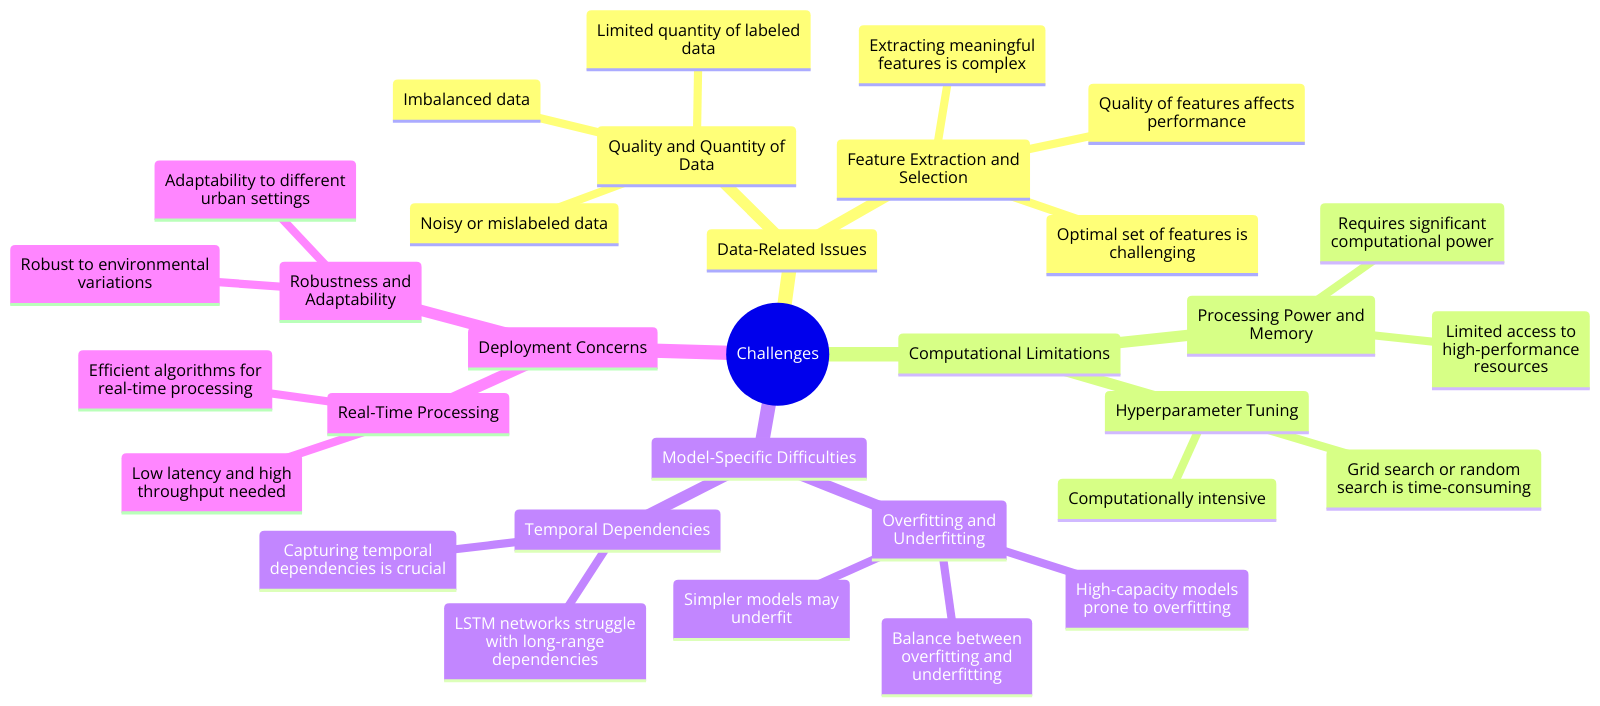
\includegraphics[width=\textwidth]{Images/challenges.png}
\caption{Challenges Encountered}
\label{fig:challenges}
\end{figure*}

\subsubsection{Real-Time Processing}
Deploying models for real-time noise classification in urban environments requires efficient algorithms that can process data quickly. Ensuring low latency and high throughput in real-time applications is challenging, particularly with resource-constrained devices like edge computing platforms.

\subsubsection{Robustness and Adaptability}
Models need to be robust to variations in environmental conditions, such as changes in background noise, recording quality, and the presence of multiple sound sources. Developing models that can adapt to different urban settings without significant performance degradation is an ongoing challenge. Conducting extensive cross-validation and robustness testing to ensure models perform well under varying conditions could be the real solution for this challenge.


By addressing these challenges, the field of urban noise classification can advance towards more accurate, efficient, and deployable solutions, contributing to better noise management and improved urban living environments.


\section{Results and Discussion}

\subsection{Introduction}

The aim of this study is to evaluate the effectiveness of various machine learning algorithms in classifying urban noise. Specifically we compared the performance of Convolutional Neural Networks (CNN),Deep Neural Networks (DNN), Long Short-Term Memory (LSTM) and Random Forest (RF) classifiers using the UrbanSound8K dataset. The models were assessed based on precision,accuracy recall and F1-score metrics.

\subsection{Results Presentation}

The performance metrics for each model are summarized in Table~\ref{tab:performance_metrics}. The DNN achieved the highest accuracy at 94.5\%, followed by the CNN at 90\%, RF at 87\%, and LSTM at 79\%.

\begin{table}[h]
\centering
\caption{Performance Metrics of Machine Learning Models}
\label{tab:performance_metrics}
\begin{tabular}{|l|c|c|c|c|}
\hline
\textbf{Model} & \textbf{Accuracy} & \textbf{Precision} & \textbf{Recall} & \textbf{F1-score} \\ \hline
DNN           & 94.5\%    & 95.1\%     & 94.0\%  & 94.6\%    \\ \hline
CNN           & 90\%      & 91.0\%     & 92.1\%  & 91.5\%    \\ \hline
Random Forest & 87\%      & 86.5\%     & 87.8\%  & 87.1\%    \\ \hline
LSTM          & 79\%      & 78.7\%     & 79.1\%  & 77.4\%    \\ \hline
\end{tabular}
\end{table}

\subsubsection{Deep Neural Networks (DNN)}

The DNN model demonstrated superior performance with the highest accuracy (94.5\%) and F1-score (94.6\%). The high precision (95.1\%) and recall (94.0\%) values indicate the DNN's effectiveness in correctly identifying and classifying urban noise types. The hierarchical learning capability of DNNs, which allows them to capture both low-level and high-level features, was a significant factor in this success.

\subsubsection{Convolutional Neural Networks (CNN)}

The CNN model performed well, achieving a 90\% accuracy. CNNs are particularly effective in extracting spatial features from audio spectrograms. The high precision (91.0\%) and recall (92.1\%) reflect the model's robustness in handling complex audio data. The convolutional layers in CNNs detect local patterns and structures in the spectrograms, enhancing their ability to classify sounds accurately.

\subsubsection{Random Forest (RF)}

The RF model achieved a commendable accuracy of 87\%, highlighting its robustness and generalization capabilities. RF's ensemble learning approach, which combines multiple decision trees, helps reduce overfitting and improve model stability. The balanced precision (86.5\%) and recall (87.8\%) values indicate the model's reliability in urban noise classification.

\subsubsection{Long Short-Term Memory Networks (LSTM)}

The LSTM model, designed to capture temporal dependencies in sequential data, achieved an accuracy of 79\%. The precision (78.7\%) and recall (79.1\%) suggest that the current architecture and preprocessing techniques might need further optimization. Despite being well-suited for sequential data, the LSTM model's performance indicates a need for better handling of long-term dependencies and potential improvements in hyperparameter tuning.

\subsection{Comparative Analysis}

Comparing the models, DNN and CNN outperformed RF and LSTM in terms of accuracy and F1-score. The DNN's deep architecture allowed it to capture intricate patterns, while the CNN's convolutional layers excelled at identifying essential features in spectrograms. The RF model demonstrated good generalization abilities, making it a practical choice for applications requiring interpretability and robustness. The LSTM model's relatively lower performance suggests the need for optimization in capturing temporal patterns.

\subsection{Implications and Interpretations}

The results underscore the effectiveness of deep learning models, particularly DNN and CNN, in urban noise classification tasks. These models leverage hierarchical and spatial feature learning capabilities to achieve high classification accuracy. The findings align with existing literature, such as the work by Bubashait and Hewahi (2021), which highlights the efficacy of CNNs and DNNs in audio classification.

The high performance of DNN and CNN models suggests that these architectures are well-suited for urban noise classification, potentially aiding in the development of robust and scalable noise monitoring systems. The RF model's balanced performance makes it a reliable choice for scenarios requiring model interpretability and robustness. Its ability to handle various types of data and provide feature importance insights is valuable for understanding the underlying data structure and making informed decisions.

The LSTM model, despite its lower performance, provides valuable insights into the importance of capturing temporal dependencies in audio data. Future work could explore hybrid models combining CNNs and LSTMs to improve performance further.

In conclusion, this study demonstrates the potential of machine learning models, particularly deep learning architectures, in addressing the challenges of urban noise classification. The findings contribute to the ongoing efforts in developing effective and efficient noise monitoring systems, ultimately enhancing urban living environments.



\section{Conclusion}

The study's main objective was to categorize urban noise utilizing Random Forest, Long Short-Term Memory networks, Convolutional Neural Networks, and Deep Neural Networks. We aimed to build models that might deliver high accuracy in the categorization of various forms of urban noise using the UrbanSound8K dataset as our target.


In terms of accuracy and F1-score, the results from the DNN and CNN models outperformed those from the RF and LSTM models. The DNN model provided the best accuracy, 94.5\%, demonstrating the ability of hierarchic learning to reflect complicated patterns in the audio data. The convolutional layers of the CNN model, which came next, were able to extract the crucial spatial characteristics from the audio spectrograms with the greatest accuracy of 90\%. With an accuracy of 87\%, the RF model demonstrated its ability to maintain a balanced approach and combine numerous decision trees to enhance generalization and minimize overfitting. With a score of 79\%, the LSTM model—which was intended to detect temporal dependencies—managed to suggest that more model tuning is necessary for the sequential audio data.


Even though the results appear promising, a number of difficulties have been encountered, such as poor data quality, computational limitations, and the need for efficient feature extraction and selection techniques. Resolving these issues is essential to enhancing the efficacy and relevance of the urban noise categorization models.

Furthermore, scalability, interaction with current urban monitoring systems, and real-time processing provide new hurdles when implementing these models in practical settings. Work has to be done on creating lightweight models that can be deployed on edge devices while taking into account very low latencies and high throughput in real-time applications.


The development of sophisticated urban noise monitoring systems will greatly benefit from the findings of this study. By addressing noise more effectively, advanced machine learning algorithms improve public health and the overall quality of life in cities. The exceptional efficacy of DNN and CNN models highlights its promise in offering precise and expandable resolutions to the urban noise categorization issue.


To sum up, this research provides insightful information about the use of machine learning in the classification of urban noise. The findings open the door for more developments in this area and emphasize how crucial it is to choose the right models depending on the demands of a certain application. To tackle the increasing problems of urban noise pollution and improve the livability of urban areas, further research and development of these approaches is needed.



\section*{List of Abbreviations}

\begin{table}[h!]
\centering
\begin{tabularx}{0.5\textwidth}{lX}
\toprule
\textbf{Abbreviation} & \textbf{Full Form} \\
\midrule
AI   & Artificial Intelligence \\
ML   & Machine Learning \\
DL   & Deep Learning \\
RF   & Random Forest \\
DNN  & Deep Neural Network \\
CNN  & Convolutional Neural Network \\
LSTM & Long Short-Term Memory \\
MFCC & Mel-Frequency Cepstral Coefficient \\
SED  & Sound Event Detection \\
WHO  & World Health Organization \\
IoT  & Internet of Things \\
\bottomrule
\end{tabularx}
\caption{List of Abbreviations}
\label{tab:abbreviations}
\end{table}






\bibliographystyle{IEEEtran}
\bibliographystyle{unsrt}
\bibliography{references}

\end{document}
